\chapter{Generalizing the Propensity Score}\label{one}

Continuous treatment variables have posed a significant challenge for causal
inference, both in the formulation and identification of scientifically
meaningful effects and in their robust estimation. Traditionally, focus has been
placed on techniques applicable to binary or categorical treatments with few
levels, allowing for the application of propensity score-based methodology with
relative ease. Efforts to accommodate continuous treatments introduced the
generalized propensity score, yet estimators of this nuisance parameter commonly
utilize parametric regression strategies that sharply limit the flexibility and
robustness of classical inverse probability weighted estimators of causal effect
parameters. We present and investigate novel, flexible estimators of the
generalized propensity score, based on a recently developed nonparametric
regression function that converges at a fast rate to the target functional.
Using our proposed estimator, we demonstrate the construction of nonparametric
inverse probability weighted estimators of a class of causal effect estimands
tailored to continuous treatments. We outline non-restrictive conditions and
selection procedures for applying undersmoothing to our generalized propensity
score estimators to develop inverse probability weighted estimators capable of
achieving the nonparametric efficiency bound, demonstrating the attainability of
these properties in numerical experiments. Open source software
implementing our proposed estimation techniques, the \texttt{haldensify}
\texttt{R} package, is briefly introduced.

\section{Introduction}\label{intro}

From the biomedical and health sciences to the social and economic sciences,
research efforts often aim to quantify the causal impacts of intervening on
continuous-valued treatments. Evaluating the causal
effects of such treatments opens the door to addressing myriad complex
scientific questions; examples include evaluating the impacts of increased
physical exercise on aging in the elderly~\citep{diaz2012population}, reductions
in surgical operating time on post-surgical health
outcomes~\citep{haneuse2013estimation}, changes in vaccination-induced
immunologic response activity on disease risk~\citep{hejazi2020efficient}, and
how total nurse hours per patient affects the risk of hosptial
readmission~\citep{mchugh2013hospitals}. The evaluation of the causal effects of
continuous treatments leads most naturally to scientific parameters that
capture dose-response phenomena, such as the well-studied \textit{causal}
dose-response curve~\citep[e.g.,][]{imbens2000role,
diaz2013targeted,kennedy2017nonparametric}.

Unfortunately, the definition of counterfactual parameters for continuous
treatments requires significant care. While counterfactual random variables
provide a formalism to describe the values an outcome measurement would have
taken if, possibly counter-to-fact, a specific level of the treatment had been
assigned (instead of that observed), for continuous treatments, the set of
enumerable counterfactuals grows quickly intractable. A prominent
simplification is coarsening, or discretization into countably few categories.
The adoption of such a strategy narrows the set of relevant counterfactual
values of the outcome variable, allowing for the subsequent straightforward
application of standard, well-studied parameters (e.g., the average treatment
effect) and corresponding well-established estimators. Despite their
convenience, such coarsening strategies come at the cost of ignoring fundamental
scientific knowledge about the system under study.

The consideration of continuous treatment variables leads to a host of
complications for the formulation, identification, and estimation of causal
effects, usually necessitating non-standard techniques for their resolution.
While the analysis of the causal dose-response curve and related estimands
brings with it many statistical challenges (e.g., a lack of asymptotic
linearity), several recent efforts have borne fruit: \citet{diaz2013targeted}
proposed a doubly robust substitution estimator of the dose-response curve's
risk, \citet{kennedy2017nonparametric} developed an estimation strategy based on
locally linear smoothing, \citet{vdl2018cvtmle} considered cross-validated
targeted minimum loss estimation of a general class of non-standard parameters
(including the dose-response curve as an example), and
\citet{westling2020causal} contributed a monotone nonparametric estimator of the
dose-response curve. These methodological advances notwithstanding, deploying
such approaches may yet require the consideration of scientifically unrealistic
counterfactual variables and infeasible intervention schedules for generating
them. Accordingly, alternative frameworks for working with continuous
treatments have been pursued.

One such framework is based on the causal effects of \textit{stochastic}
interventions~\citep{stock1989nonparametric, diaz2012population,
haneuse2013estimation, vanderweele2013causal, young2014identification}, which
consider setting the post-intervention treatment level to a random draw from a
user-specified distribution. This approach makes for a highly flexible means of
defining counterfactual random variables --- indeed, even static interventions
are a special case in which the post-intervention treatment value is drawn from
a degenerate distribution with all mass placed on a single treatment level. To
ensure scientifically meaningful counterfactuals, careful attention must be paid
to defining the particular distribution from which the post-intervention
treatment value is drawn. A popular strategy draws post-intervention treatment
values from a modification of the natural treatment distribution.
Counterfactuals defined in this way may be better aligned with plausible future
interventions that may be scientifically engineered. Recent efforts have
provided several candidate approaches~\citep{diaz2012population,
haneuse2013estimation, young2014identification, kennedy2019nonparametric} for
identifying and estimating the causal effects of stochastic interventions. The
framework of stochastic interventions is further distinguished by its
generalizability, which has allowed for recent extensions to complex settings
involving mediating variables~\citep{diaz2020causal, diaz2020nonparametric,
hejazi2020nonparametric}.

While stochastic interventions appear a promising avenue, estimation strategies
formulated within this framework run aground of a familiar issue: evaluation of
the \textit{generalized} propensity score~\citep{austin2018assessing} (i.e.,
conditional treatment density given covariates), analogous to the propensity
score~\citep{rosenbaum1983central}, is required. The generalized propensity
score has been a common ingredient for evaluating the causal effects of
continuous treatments, both within and without the stochastic intervention
framework. For example, \citet{robins2000marginal} posited a marginal structural
model of the outcome process and used inverse probability weighted estimation of
its parameters, which include the generalized propensity score. Avoiding direct
modeling of the outcome, \citet{hirano2004propensity} formulated an adjustment
procedure, based on covariate-balancing, for estimation of the generalized
propensity score. Along similar lines, \citet{imai2004causal} considered direct
extensions of the propensity score to multi-level treatments, while
\citet{galvao2015uniformly} proposed a two-step semiparametric-efficient
estimator utilizing inverse weighting based on the generalized propensiy score.
Despite its prevalence, most proposals rely upon restrictive parametric modeling
assumptions to facilitate estimation of the generalized propensity score,
though, more recently, flexible estimators leveraging advances in machine
learning have received relatively meager attention~\citep{diaz2011super,
zhu2015boosting}.

In the present work, we discuss several flexible semiparametric strategies for
estimation of the generalized propensity score, all presented within the context
of evaluating the causal effects of stochastic interventions on continuous
treatments. From among these proposals, we highlight a nonparametric estimator
of the conditional treatment density based on pooled hazard regression. Building
upon our proposed generalized propensity score estimator, we develop and
evaluate a unique inverse probability weighted estimator capable of achieving
levels of efficiency usually attainable only with doubly robust estimation
frameworks. We additionally discuss open source software packages,
\texttt{haldensify}~\citep{hejazi2021haldensify} and
\texttt{sl3}~\citep{coyle2021sl3}, for the \texttt{R} statistical programming
environment~\citep{R}, that facilitate implementation of our generalized
propensity score estimators and efficient inverse probability weighted
estimators.

%%%%%%%%%%%%%%%%%%%%%%%%%%%%%%%%%%%%%%%%%%%%%%%%%%%%%%%%%%%%%%%%%%%%%%%%%%%%%%%
\section{Preliminaries}\label{one_prelim}

\subsection{Problem Formulation and Notation}\label{setup}

Let $W \in \mathcal{W}$ denote a vector of baseline covariates, $A \in
\mathcal{A}$ a real-valued continuous treatment, and $Y \in \mathcal{Y}$ an
outcome of interest. To formalize the causal question of interest, we introduce
a nonparametric structural equation model (NPSEM) to describe the
data-generating process~\citep{pearl2009causality}. Specifically, we assume the
following system of structural equations generates the observed data:
\begin{equation*}\label{npsem}
  W = f_W(U_W); A = f_A(W, U_A); Y = f_Y(A, W, U_Y),
\end{equation*}
where $\{f_W, f_A, f_Y\}$ are deterministic functions, and $\{U_W, U_A, U_Y\}$
are exogenous random variables. Importantly, the NPSEM implies a model for the
distribution of counterfactual random variables, which are generated by specific
interventions on the data-generating process. Within the framework of potential
outcomes~\citep{neyman1938contribution, rubin1978bayesian,
rubin1980randomization, rubin2005causal}, the full (unobserved) data unit may be
expressed $X = (W, Y_a: a \in \mathcal{A})$, where the counterfactuals $Y_a$
represent outcomes corresponding to each possible value in the support of the
treatment $\mathcal{A}$. Our focus will be the estimation of counterfactual
treatment parameters that are themselves functionals of $X$.

Consider the observed data as having been generated by typical cohort sampling,
where the data on a single observational unit $O$ is denoted $O = (W, A, Y)$. We
use $P_0$ to denote the distribution of $O$, and, assuming access to $n$
independent copies of $O$, $P_n$ for the empirical distribution of the $n$
copies $O_1, \ldots, O_n$. Assuming only that $P_0$ is an element of the
nonparametric statistical model $\mathcal{M}$, i.e., $P_0 \in \mathcal{M}$, we
avoid placing any restrictions on the form of $P_0$. We use $p_0$ to denote the
density of $O$, which evaluated on a typical observation $o$, is
\begin{equation*}\label{likelihood_factorization}
  p_0(o) = q_{0,Y}(y \mid A = a, W = w) g_{0,A}(a \mid W = w) q_{0,W}(w) \ ,
\end{equation*}
where $q_{0, Y}$ denotes the conditional density of $Y$ given $\{A, W\}$ with
respect to some dominating measure, $g_{0, A}$ the conditional density of $A$
given $W$ with respect to dominating measure $\mu$, and $q_{0, W}$ the density
of $W$ with respect to dominating measure $\nu$.

Counterfactual quantities of interest may be defined by specific interventions
that alter the structural equation $f_A$ and insert post-intervention treatment
values of interest in place of the values that would be naturally generated by
$f_A$. A familiar example comes in the form of \textit{static interventions},
which are defined by replacing $f_A$ with a specific value, selected \textit{a
priori}, $a \in \mathcal{A}$. When the cardinality of $\mathcal{A}$ is small ---
that is, there are few treatment values --- contrasts of the counterfactual
means of static interventions under each $a \in \mathcal{A}$ can prove useful.
On the other hand, when the cardinality of $\mathcal{A}$ is large, or when $A$
is continuous-valued, the evaluation of many such counterfactual means is of
questionable scientific relevance and, besides, statistically challenging.

A \textit{stochastic intervention} modifies the value $A$ would naturally
assume, $f_A(W, U_A)$, by replacing it with a draw from a post-intervention
distribution $\tilde{g}_{0,A}(\cdot \mid W)$ (n.b., the zero subscript
emphasizes that this distribution may depend on the true, but unknown,
data-generating distribution $P_0$). Of course, a stochastic intervention may be
designed to collapse into a static intervention simply by selecting the
post-intervention distribution $\tilde{g}_{0,A}(\cdot \mid W)$ to be degenerate,
so as to place all mass on a single point $a \in \mathcal{A}$.

\citet{diaz2012population} described a stochastic intervention that draws $A$
from a distribution such that $\tilde{g}_{0,A}(a \mid W) = g_{0,A}(d^{-1}(a, w)
\mid W)$, indexed by a user-supplied \textit{shifting} function, and
a given $a \in \mathcal{A}$. Shortly thereafter, \citet{haneuse2013estimation}
showed that estimation of the causal effect of this shifting intervention is
equivalent to that of an intervention modifying the value $A$ would naturally
assume according to a regime $d(A,W)$ under the assumption of
\textit{piecewise smooth invertibility}:
\begin{assumptioniden}[Piecewise smooth invertibility]\label{ass:one_inv}
  For each $w \in \cal W$, assume that the interval
  ${\cal I}(w) = (l(w,), u(w))$ may be partitioned into subintervals
  ${\cal I}_{\delta,j}(w):j = 1, \ldots, J(w)$ such that $d(a, w)$ is equal to
  some $d_j(a, w)$ in ${\cal I}_{\delta,j}(w)$ and $d_j(\cdot,w)$ has inverse
  function $h_j(\cdot, w)$ with derivative $h_j'(\cdot, w)$.
\end{assumptioniden}
Assumption~\ref{ass:one_inv} can be used to show that the intervention may be
interpreted on the individual level~\citep{young2014identification}.
Importantly, the regime $d(A,W)$ may depend on both covariates $W$ and the
treatment $A$ that would be assigned in the absence of the regime; consequently,
this has been termed a \textit{modified treatment policy} (MTP). Both
\citet{haneuse2013estimation} and \citet{diaz2018stochastic} were motivated by
counterfactual questions of modifying an intervention, the former seeking to
evaluate the effect on patient health of reducing surgical operating time and
the latter by the effect of adjusting prescribed exercise regimens based on the
athletic habits of patients. Conveniently, both sets of authors considered an
MTP of the form
\begin{equation}\label{eqn:one_defn_shift}
  d(a, w) =
  \begin{cases}
    a + \delta(w) & \text{if } a + \gamma \leq u(w) \\
    a & \text{if } a + \gamma > u(w)
  \end{cases},
  \text{where} \quad \delta(w) = \gamma \in \R
\end{equation}
and $u(w)$ is the maximum value in the conditional support of $g_{0,A}(\cdot
\mid W = w)$. This intervention generates a counterfactual random variable
$Y_{d(A, W)} \coloneqq f_Y(d(A, W), W, U_Y)$ whose distribution we denote
$P_0^{\delta}$. The goal, then, is to estimate $\psi_{0, \delta} \coloneqq
\E_{P_0^{\delta}} \{ Y_{d(A, W)} \}$, the mean of this counterfactual outcome.

\subsection{Identifying the Population Intervention Effect}\label{one_pie_param}

\citet{diaz2012population} introduced the \textit{population intervention
effect} (PIE) $\theta_{0, \delta} \coloneqq \psi_{0, \delta} - \E Y$. As $\E Y$
is trivially estimable from the observed data, their efforts focused on
identification and estimation of $\psi_{0,\delta}$. In particular, these authors
showed that $\psi_{0, \delta}$ is identified by
\begin{align}\label{eqn:ident_pie_2012}
  \psi_{0,\delta} &= \int_{\mathcal{W}} \int_{\mathcal{A}}
  \overline{Q}_{0,Y}(a, w) g_{0, A}(d^{-1}(a, w) \mid W = w)
  q_{0, W}(w) d\mu(a)d\nu(w) \nonumber \\
  &= \int_{\mathcal{W}} \int_{\mathcal{A}}
  \overline{Q}_{0,Y}(d(a, w), w) g_{0, A}(a \mid W = w)
  q_{0, W}(w) d\mu(a)d\nu(w)
\end{align}
where $\overline{Q}_{0,Y}(a,w) \coloneqq \E_{P_0}[Y \mid A = a, W = w]$, the
conditional mean of $Y$ given $A = a$ and $W = w$, as implied by $P_0$, and
$g_{0,A}(a \mid W = w)$ is the conditional density of the treatment. For the
statistical functional given in equation~\eqref{eqn:ident_pie_2012} to
correspond to the causal estimand of interest, several untestable assumptions
are required, including
% Identification assumptions
\begin{assumptioniden}[Lack of interference]
  Assume $Y^{d(a_i, w_i)}_i \indep d(a_j, w_j)$ for $i \neq j$.
  \label{ass:interfere_one}
\end{assumptioniden}
\begin{assumptioniden}[Consistency]
  Assume $Y^{d(a, w)} = Y$ in the event $A = d(a, w)$.
  \label{ass:consist_one}
\end{assumptioniden}
\begin{assumptioniden}[No unmeasured confounding]
  Assume $A \indep Y^{d(a, w)} \mid W = w$.
  \label{ass:nuc_one}
\end{assumptioniden}
\begin{assumptioniden}[Positivity]
  Assume $a \in \mathcal{A} \implies d(a, w) \in \mathcal{A} \mid
  W = w$ for all $w \in \mathcal{W}$.
  \label{ass:pos_one}
\end{assumptioniden}
Together, assumptions~\ref{ass:interfere_one} and~\ref{ass:consist_one} are often
referred to as the stable unit treatment value assumption
(SUTVA)~\citep{rubin1978bayesian,rubin1980randomization}. The positivity
assumption~\ref{ass:pos_one}, required to establish
equation~\eqref{eqn:ident_pie_2012}, is unlike its analog for simpler (i.e.,
static or dynamic) intervention schedules. Instead of requiring positive mass to
be placed across all treatment levels for all covariate strata $w \in
\mathcal{W}$, this positivity assumption requires only that the
post-intervention treatment mechanism be bounded, i.e., $\prob_{P_0}
\{g_{0,A}(d^{-1}(A, W) \mid W) / g_{0,A}(A \mid W) > 0 \} = 1$, which may
generally be satisfied by a suitable choice of the parameter $\delta(W)$ in the
treatment modification function $d(A,W)$.

Beyond their careful study of the identification of this causal effect,
\citet{diaz2012population, diaz2018stochastic} derived the \textit{efficient
influence function} (EIF), a quantity central to semiparametric efficiency
theory, of $\psi_{0, \delta}$ with respect to the nonparametric statistical
model $\M$. Using the EIF, these authors proposed efficient estimators
constructed based on the form of the EIF. When evaluated on a typical
observation $o$, a suitable expression for the EIF is
\begin{equation}\label{eqn:one_eif_full}
  D^{\star}(P_0)(o) = H(a, w)\{y - \overline{Q}_{0,Y}(a, w)\} +
  \overline{Q}_{0,Y}(d(a, w), w) - \psi_{0,\delta},
\end{equation}
where the auxiliary covariate $H(a,w)$ takes the form $H(a, w) = g_{0,
A}(d^{-1}(a, w) \mid w) / g_{0, A}(a \mid w)$. The EIF characterizes the best
possible asymptotic variance, or efficiency bound, of all regular asymptotically
linear estimators of $\psi_{0, \delta}$ and may thus be used in the development
of efficient estimation strategies.

\subsection{Estimating the Population Intervention Effect}\label{pie_est}

To facilitate estimation of $\psi_{0,\delta}$, \citet{diaz2018stochastic}
defined a direct (or, substitution) estimator based on the G-computation
formula. This classical estimator is of the form
\begin{align}\label{eqn:plugin}
  \psi_{n,\delta}^{\text{SUB}} \coloneqq&
      \int \overline{Q}_{n,Y}(d(a, w), w) dQ_{n,AW}(a,w) \nonumber \\
      =& \frac{1}{n} \sum_{i=1}^n \overline{Q}_{n,Y}(d(A_i, W_i), W_i)\ ,
\end{align}
where $Q_{n,AW}(a,w)$ is an estimate of the joint distribution of $(A,W)$ based
on the empirical distribution. An inverse probability weighted (IPW) estimator
of $\psi_{0,\delta}$ takes the form
\begin{equation}\label{eqn:ipw}
  \psi_{n,\delta}^{\text{IPW}} = \frac{1}{n} \sum_{i=1}^n \frac{g_{n, A}
    (d^{-1}(A_i, W_i) \mid W_i)}{g_{n, A}(A_i \mid W_i)} Y_i \ .
\end{equation}
In both equations~\eqref{eqn:plugin} and~\eqref{eqn:ipw}, as well as in the
sequel, the subscript $n$ denotes the use of estimated quantities in lieu of
their true counterparts --- that is, $g_{n,A}$ is simply an estimate of the
conditional treatment density $g_{0,A}$, while $\overline{Q}_{n,Y}$ is an
estimate of the outcome mechanism $\overline{Q}_{0,Y}$. Both the direct
estimator $\psi_{n,\delta}^{\text{SUB}}$ and the IPW estimator
$\psi_{n,\delta}^{\text{IPW}}$ require estimation of only a single nuisance
parameter (the outcome mechanism and the conditional treatment density,
respectively) but are well-known to be irregular, fail to be asymptotically
consistent, or fail to achieve the semiparametric efficiency bound. What's more,
neither estimator is asymptotically linear for $\psi_{0,\delta}$ when flexible
regression strategies are used for nuisance parameter estimation, significantly
limiting the scenarios in which these approaches may be successfully applied.

Two popular frameworks for efficient estimation, both taking advantage of the
EIF, include one-step
estimation~\citep{pfanzagl1985contributions,bickel1993efficient} and targeted
minimum loss-based (TML) estimation~\citep{vdl2006targeted, vdl2011targeted,
vdl2018targeted}. Importantly, both the one-step and TML estimators are
\textit{doubly robust}, a property which affords two important conveniences.
Firstly, both estimators are consistent for $\psi_{0,\delta}$ when either of the
initial estimates of $g_{n,A}$ and $\overline{Q}_{n,Y}$ are consistent for their
respective targets; however, these estimators only achieve asymptotic efficiency
when \textit{both} initial estimates are consistent. Secondly, as a consequence
of their explicit construction based on the EIF, both readily accommodate the
use of flexible, data-adaptive estimation strategies for the initial estimation
of nuisance parameters. This latter property provides these estimators with
a distinct advantage over their substitution and IPW estimator counterparts: two
opportunities to avoid model misspecification from restrictive (e.g.,
parametric) modeling strategies.

Invoking either estimation strategy proceeds first by constructing initial
estimates, $g_{n,A}$ and $\overline{Q}_{n,Y}$, of the conditional treatment
density $g_{0,A}$ and the outcome mechanism $\overline{Q}_{0,Y}$. The two
approaches diverge at their second stage, which focuses on bias correction. In
the one-step framework, this amounts to updating the initial substitution-based
estimate $\psi_{n,\delta}$ by adding to it the empirical mean of the estimated
EIF. In the TML estimation framework, a univariate (often, logistic) parametric
tilting model is used to update the initial estimate $\overline{Q}_{n,Y}$ of the
outcome mechanism in such a way that the EIF estimating equation is solved to
a desirable degree. Plugging this updated initial estimate into the substitution
formula given in equation~\eqref{eqn:plugin} results in a targeted estimator of
$\psi_{0,\delta}$.

As both the one-step and TML estimation procedures require the EIF, we recall
that an estimate of the EIF may be constructed from
equation~\eqref{eqn:one_eif_full} by plugging in initial estimates of nuisance
parameters. The estimated EIF, evaluated on observation $i$, is
\begin{equation*}
  D^{\star}_{n,i} \coloneqq H_n(A_i, W_i) \{Y_i -
  \overline{Q}_{n,Y}(A_i, W_i)\} +
  \overline{Q}_{n,Y}(d(A_i, W_i), W_i) - \psi_{n,\delta} \
\end{equation*}
with auxiliary term $H_n(a,w) \coloneqq g_{n,A}(d^{-1}(a, w) \mid w) /
g_{n,A}(a \mid w)$. Using the estimated EIF $D^{\star}_{n,i}$, the one-step
estimator may then be defined
\begin{equation}\label{eqn:one_step}
  \psi_{n,\delta}^{+} \coloneqq \psi_{n,\delta} + \frac{1}{n} \sum_{i=1}^n
   D^{\star}_{n,i} \ .
\end{equation}
Similarly, an asymptotically linear TML estimator may be constructed by updating
the initial estimator $\overline{Q}_{n,Y}$ to a tilted variant
$\overline{Q}_{n,Y}^{\star}$, through a logistic tilting model of the form
$\logit \overline{Q}_{n,Y}^{\star} = \logit \overline{Q}_{n,Y} + \epsilon
H_n$, in which the initial estimate $\overline{Q}_{n,Y}$ is taken as an
offset and only the parameter $\epsilon$ need be estimated. The targeted plug-in
estimator is then
\begin{equation}\label{eqn:tmle}
  \psi_{n,\delta}^{\star} \coloneqq \int
  \overline{Q}_{n,Y}^{\star}(d(a, w), w) dQ_{n,AW}(a,w) \ .
\end{equation}
Both of these efficient estimators depend on initial estimates of the nuisance
functions $(\overline{Q}_{n,Y}, g_{n,A})$. Throughout, we focus on developing
improved estimators $g_{n,A}$ of the generalized propensity score $g_{0,A}$,
ultimately towards the goal of facilitating the construction of enhanced
efficient estimators of $\psi_{0, \delta}$.

\subsection{The Highly Adaptive Lasso Estimator}\label{one_hal_est}

In our subsequent developments, we make use of a recently developed
nonparametric regression function, the highly adaptive lasso
(HAL)~\citep{vdl2017generally, vdl2017uniform}. The HAL estimator approximates
a functional parameter of interest using a linear combination of basis
functions, with the requirement that the target functional parameter belong to
the set of c\`{a}dl\`{a}g (i.e., right-hand continuous with left-hand limits)
functions with sectional variation norm bounded by a finite (but unknown)
constant, a global smoothness restriction that limits the degree of variability
that the target functional may exhibit. Similarly positioned approaches in
nonparametric estimation generally require more restrictive local smoothness
assumptions. For example, minimax convergence rates achieved under the
assumption that the target functional belongs to a smoothness class
characterized by H{\"o}lder balls~\citep[e.g.,][]{robins2008higher,
robins2017minimax} are compromised by the failure of resultant function classes
to exclude from admissibility highly erratic functions (e.g., the Weierstrass
function, which falls in the class of H{\"o}lder-$\alpha$ functions for $\alpha
< 1$ and $d = 1$).

For any function $f \in \mathcal{D}[0,\tau]$, the Banach space of $d$-variate
real-valued c\`{a}dl\`{a}g functions on a cube $[0,\tau] \in \R^d$, the
sectional variation norm of $f$ may be expressed
\begin{equation*}
  \lVert f \rVert^{\star}_\nu \coloneqq \lvert f(0) \rvert + \sum_{s
  \subset\{1, \ldots, d\}} \int_{0_s}^{\tau_s} \lvert df_s(u_s) \rvert,
\end{equation*}
where $s$ are subsets of $\{0, 1, \ldots, d\}$, defined by partitioning
$[0,\tau]$ in $\{0\} \{ \cup_s (0_s,\tau_s]\}$, and the sum is taken over all
subsets of the coordinates $\{0,1,\ldots,d\}$. For a given subset $s \subset
\{0,1,\ldots,d\}$, define $u_s = (u_j : j \in s)$ and $u_{-s}$ as the complement
of $u_s$; then, $f_s: [0_s, \tau_s] \rightarrow \R$, defined as $f_s(u_s)
= f(u_s,0_{-s})$. Thus, $f_s(u_s)$ is a section of $f$ that sets the components
in the complement of $s$ to zero, that is, allowing variation only along
components in $u_s$.
%Perhaps interestingly, there is a close correspondence between this definition
%of variation norm and the notion of Hardy-Krause
%variation~\citep{qiu2020universal, owen2005multidimensional}.

\citet{vdl2015generally, vdl2017generally} proved that the HAL estimator
converges to the target functional at a rate faster than $n^{-1/4}$, without any
contribution from the dimensionality $d$ of the problem at hand, so long as $d$
remains fixed. Subsequent theoretical investigations improved this rate of
convergence to $n^{-1/3} \log(n)^{d/2}$~\citep{bibaut2019fast}, with ongoing
work yielding promising further improvements still. The HAL estimator can be
thought of as proceeding in two general steps. Firstly, a rich set of indicator
(or higher-order, i.e., spline) basis functions are generated to represent the
target functional; this step is a mapping of the covariate space in terms of the
HAL basis. Subsequently, lasso regression~\citep{tibshirani1996regression} is
applied to a linear combination of these basis functions, minimizing the
expected value of an appropriately chosen loss function while constraining the
$L_1$-norm of the vector of coefficients to be bounded by a finite constant
matching the sectional variation norm of the HAL representation of the target
functional. \citet{benkeser2016highly} first demonstrated the utility of the HAL
estimator in an extensive series of numerical experiments. The HAL estimator is
implemented in the free and open source \texttt{hal9001}
package~\citep{coyle2021hal9001, hejazi2020hal9001} for the \texttt{R}
language and environment for statistical computing~\citep{R}.

When a nuisance parameter of interest is taken as the target functional, the HAL
estimator may be applied to generate initial estimates, under the assumption
that the true nuisance parameter functional (e.g., the generalized propensity
score) be of finite sectional variation. When the nuisance parameter $\eta$,
with arbitrary input $Z$, is real-valued, its HAL representation may be
expressed
\begin{align}\label{eq:hal}
  \eta(z) &= \eta(0) + \sum_{s \subset\{1,\ldots,d\}} \int_{0_s}^{z_s} d
  \eta_s(u_s) \nonumber \\ & = \eta(0) + \sum_{s \subset\{1,\ldots,d\}}
  \int_{0_s}^{\tau_s} \mathbb{I}(u_s \leq z_s) d \eta_s(u_s),
\end{align}
which can be approximated by the use of a discrete measure placing mass on each
observed $Z_{s,i}$. When the range of $\eta$ is the unit interval, an analogous
approach, using instead $\logit \eta$, may be pursued based on a representation
of~\citet{gill1995inefficient}; \citet{ertefaie2020nonparametric} work with this
representation in using HAL regression for estimation of the propensity score
for binary treatments. Now, take $z_{s,i}$ to be support points of $\eta_s$ and
let $\phi_{s,i}(c_s) \coloneqq \mathbb{I}(z_{s,i} \leq c_s)$, then
\begin{equation*}
 \eta_\beta = \beta_0 + \sum_{s \subset\{1,\ldots,d\}} \sum_{i=1}^{n}
   \beta_{s,i} \phi_{s,i},
\end{equation*}
where $\lvert \beta_0 \rvert + \sum_{s \subset\{1,\ldots,d\}} \sum_{i=1}^{n}
\lvert \beta_{s,i} \rvert$ is an approximation of the sectional variation norm
of $\eta$. The loss-based HAL estimator $\beta_n$ may then be defined
\begin{equation*}
  \beta_{n, \lambda} = \argmin_{\beta: \lvert \beta_0 \rvert + \sum_{s
  \subset\{1,\ldots,d\}} \sum_{i=1}^{n} \lvert \beta_{s,i} \rvert <\lambda} P_n
  L(\eta_{\beta}),
\end{equation*}
where $P_n f = n^{-1} \sum_{i = 1}^n f(O_i)$ and $L(\cdot)$ is an appropriately
chosen loss function; see~\citet{dudoit2005asymptotics} for an illuminating
discussion of appropriate choices of loss function for a range of loss-based
estimation problems. Salient to our goal of estimating the generalized
propensity score, the negative log-likelihood loss, $L(\eta) = -\log(p_{\eta})$,
is a suitable loss function for density estimation. Finally, the HAL estimate of
$\eta$ may be denoted $\eta_{n,\lambda} \equiv \eta_{\beta_{n, \lambda}}$. Each
choice of the regularization term $\lambda$ corresponds to a unique HAL
estimator, though, generally speaking, methods for the selection of $\lambda$
must be tailored to the estimation goal in order to yield suitable candidate
estimators.

%%%%%%%%%%%%%%%%%%%%%%%%%%%%%%%%%%%%%%%%%%%%%%%%%%%%%%%%%%%%%%%%%%%%%%%%%%%%%%%
\section{Estimating the Generalized Propensity Score}\label{methods}

We now turn to procedures for estimation of the generalized propensity score
$g_{0,A}$, from which we may be able to subsequently develop efficient,
nonparametric estimators of $\psi_{0,\delta}$. As will be demonstrated in the
sequel, both conditional density estimators are flexible, allowing for the use
of arbitrary, data-adaptive regression methods to be leveraged. For
compatibility with our subsequent theoretical results, we present our
conditional density estimation procedures using the HAL estimator discussed in
Section~\ref{one_hal_est}; this is chiefly for three reasons. Firstly, formal
theory guarantees a suitable convergence rate, for estimator construction, when
the HAL estimator is used to approximate a nuisance functionals. Secondly,
contemporaneous efforts have made headway in developing efficient direct and IPW
estimators of low-dimensional parameters in causal inference
settings~\citep{vdl2019efficient,ertefaie2020nonparametric}. Thirdly, the
algorithm is readily available in the free and open source \texttt{hal9001}
\texttt{R} package~\citep{coyle2021hal9001, hejazi2020hal9001}.

In considering estimation of $g_{0,A}$, a straightforward strategy involves
assuming a parametric working model for relevant moments of the density
function, allowing the use of standard regression techniques to generate
suitable estimates~\citep{robins2000marginal,
hirano2004propensity,imai2004causal}. For example, one could operate under the
working assumption that the density of $A$ given $W$ follows a Gaussian
distribution with homoscedastic variance and mean $\sum_{j=1}^p \beta_j
\phi_j(W)$, where $\phi = (\phi_j : j)$ are user-specified basis functions and
$\beta = (\beta_j : j)$ are unknown regression parameters. Under such a regime,
a density estimate could be generated by fitting a linear regression of $A$ on
$\phi(W)$ to estimate $\E[A \mid W]$, paired with maximum likelihood estimation
of the variance of $A$. In this case, the estimated conditional density would be
given by the density of a Gaussian distribution evaluated at these estimates.
While a reasonable approach, such a strategy makes strong parametric assumptions
about the form of the conditional density function and may, on this account, be
more prone to model misspecification than alternative strategies that make fewer
such assumptions.

Constructing a flexible density estimator is a more challenging problem, as the
set of available tools is considerably limited. These limitations motivated our
investigations of novel conditional density estimators capable of incorporating
arbitrary regression functions. We describe two such classes of estimators in
the sequel, with implementations of these proposals provided in the free and
open source \texttt{sl3} and \texttt{haldensify} \texttt{R}
packages~\citep{coyle2021sl3, hejazi2021haldensify}, respectively.

\subsection{Semiparametric Location-Scale Estimators}\label{hose_hese_est}

A recently developed family of flexible semiparametric conditional density
estimators takes the general form $\rho(A - \mu(W) / \sigma(W))$, where $\rho$
is a given marginal density function. Conditional density estimation procedures
falling within this framework may be characterized as belonging to
a \textit{conditional location-scale} family, i.e., where $g_{n,A}(A \mid W)
= \rho((A - \mu_n(W)) / \sigma_n(W))$; where we stress that the marginal density
mapping $\rho$ is selected \textit{a priori}, leaving only the relevant moments
$\mu$ and $\sigma$ to be estimated.

Though the restriction to (conditional) location-scale families imposes some
limitations on the form of the target functional, the strategy is made
particularly flexible by its ability to incorporate arbitrary, data-adaptive
regression strategies for the estimation of $\mu(W) = \E[A \mid W]$ and,
optionally, of the conditional variance $\sigma(W) = \E[(A - \mu(W))^2 \mid W]$.
In particular, in settings with limited data, the additional structure imposed
by the assumption of form of the target density functional (i.e., in the
specified kernel function $\rho$) can prove beneficial, when the true density
function admits such a representation. While we stress that this procedure is
surely not a novel contribution of the present work, we have been otherwise
unable to ascertain a formal description of it; thus, we provide such
a formalization in Algorithm~\ref{alg:loc_scale_dens}, which sketches the
construction of conditional density estimators of this family.\\

\begin{algorithm}[H]
\label{alg:loc_scale_dens}
\SetAlgoLined
\KwResult{Estimates of the conditional density of $A$, given $W$.}
\SetKwInOut{Input}{Input}\SetKwInOut{Output}{Output}
\Input{
  \begin{itemize}
    \item[] An observed data vector of the continuous treatment for $n$
      units: $A$
    \item[] An observed data vector (or matrix) of the baseline covariates for
      $n$ units: $W$
    \item[] A kernel function specification to be used to construct the density
       estimate: $\rho$
    \item[] A candidate regression procedure to estimate the conditional mean
      $\mu(W)$: $f_{\mu}$
    \item[] A candidate regression procedure to estimate the
       conditional variance $\sigma(W)$: $f_{\sigma}$
  \end{itemize}
}
\BlankLine
\begin{enumerate}
\itemsep4pt
\item Estimate $\E[A \mid W]$, the conditional mean of $A$ given $W$, by
  applying the regression estimator $f_{\mu}$, yielding $\hat{\mu}(W)$.
\item Estimate $\mathbb{V}[A \mid W]$, the conditional variance of $A$ given
  $W$, by applying the regression estimator $f_{\sigma}$, yielding
  $\hat{\sigma}^2(W)$. Note that this step involves only estimation of the
  conditional mean $\E[(A - \hat{\mu}(W))^2 \mid W]$.
\item Estimate the one-dimensional density of $(A - \hat{\mu}(W))^2
  / \hat{\sigma}^2(W)$, using kernel smoothing to obtain $\hat{\rho}(A)$.
\item Construct the estimated conditional density $g_{n,A}(A \mid W)
  = \hat{\rho}((A - \hat{\mu}(W)) / \hat{\sigma}(W))$.
\end{enumerate}
\BlankLine
\Output{$g_{n,A}$, an estimate of the generalized propensity score.}
\caption{Location-scale conditional density estimation}
\end{algorithm}

The sketch of the algorithm for constructing estimators $g_{n,A}(a \mid w)$ of
the generalized propensity score may take two forms, which diverge at the second
step above. Firstly, one may elect to estimate only the conditional mean
$\mu(W)$ via a regression technique, leaving the variance to be taken as
constant (estimated simply as the marginal mean of $\E[(A - \hat{\mu}(W))^2]$).
Estimators of this form may be described as having \textit{homoscedastic error},
based on the variance assumption made. Alternatively, one may additionally
estimate the conditional variance $\sigma^2(W)$ via the residuals of the
estimated conditional mean, that is, estimating instead the conditional mean
$\E[(A - \hat{\mu}(W))^2 \mid W]$.

While the regression procedures $f_{\mu}$ and $f_{\sigma}$ used to estimate the
conditional mean $\mu(W)$ and the conditional variance $\sigma^2(W)$,
respectively, may be arbitrary, with candidates including, for example, random
forests~\citep{breiman2001random}, spline regression~\citep{stone1994use,
friedman1991multivariate}, or regression ensembles~\citep{wolpert1992stacked,
breiman1996stacked,vdl2007super}, we recommend the use of HAL
regression~\citep{benkeser2016highly,vdl2017generally}, as its use will ensure
an enhanced rate of convergence~\citep{bibaut2019fast} of the estimator
$g_{n,A}$ to its target $g_{0,A}$. The data-adaptive nature of HAL regression
affords a degree of flexibility that ought to limit opportunities for model
misspecification to compromise estimation of $g_{0,A}$; morever, their improved
convergence rate will help to facilitate the construction of asymptotically
linear, and possibly efficient, estimators of $\psi_{0, \delta}$.

\subsection{Nonparametric Hazard Regression Estimator}\label{pooled_haz_est}

Estimators that eschew any assumptions on the form of the conditional density
are a rarity. Notably, \citet{diaz2011super} gave a proposal for constructing
semiparametric estimators of this target quantity based on exploitation of the
relationship between the (conditional) hazard and density functions. Our
proposal builds upon theirs, replacing the original recommendation of an
arbitrary classification model with the HAL regression function. This
contribution requires the key change of adjusting the penalization aspect of HAL
regression to respect the use of a loss function appropriate for prediction on
the hazard scale, i.e., $-\log g_{n,A}$~\citep{dudoit2005asymptotics}. As
a consequence of this adjustment, the resultant conditional density estimator
is made capable of incorporating sample-level weights.

To build an estimator of a conditional density, \citet{diaz2011super} considered
discretizing the observed $A \in \mathcal{A}$ based on a number of bins $T$ and
a binning procedure (e.g., equally distributing observed mass across each of the
$T$ bins or forcing each of the $T$ bins to be of the same length). The choice
of the tuning parameter $T$ corresponds conceptually to the choice of bandwidth
in classical kernel density estimation. To take an example, an instantiation of
this procedure would divide the observed support of $A$ into, say, $T = 7$, bins
of equal length. Such a partitioning would require $T + 1$ cutpoints along
the support of $A$, yielding $T$ bins: $[\alpha_1, \alpha_2), [\alpha_2,
\alpha_3), \ldots, [\alpha_6, \alpha_7), [\alpha_7, \alpha_8]$. Next, relevant
components of the observed data $\{A_i, W_i\}_{i=1}^n$ would be reformatted such
that each observational unit $\{A_i, W_i\}$ would be represented by a set of up
to $T$ records, with the number of records for a given unit matching the
position of the bin into which the observed $A_i$ falls. For clarity, consider
an individual unit $\{A_i, W_i\}$ for which the value $A_i$ falls in the fifth
bin of the seven into which the support has been partitioned (i.e., $[\alpha_5,
\alpha_6)$). Five distinct records would be used to represent the data on this
single unit: $\{A_{ij}, W_{ij}\}_{j=1}^5$, where $\{\{A_{ij} = 0\}_{j=1}^4$,
$A_{i5} = 1\}$ and five exact copies of $W_i$, $\{W_{ij}\}_{j=1}^5$. This
representation as multiple records allows for the hazard probability of $A_i$
belonging to a particular bin along the discretized support to be evaluated via
standard classification techniques. In fact, this proposal reformulates the
classification problem into a corresponding set of hazard regressions:
\begin{align*}
   \prob (A \in [\alpha_{t-1}, \alpha_t) \mid W) = &\prob (A \in [\alpha_{t-1},
   \alpha_t) \mid A \geq \alpha_{t-1}, W) \\ &\times  \prod_{j = 1}^{t -1} \{1
   - \prob (A \in [\alpha_{j-1}, \alpha_j) \mid A
   \geq \alpha_{j-1}, W) \},
\end{align*}
where the probability of $A \in \mathcal{A}$ falling in a bin $[\alpha_{t-1},
\alpha_t)$ may be directly estimated from any arbitrary binary regression model,
since the likelihood of this model may be re-expressed in terms of the
likelihood of a binary variable in a data set expressed through a repeated
measures structure.

Specifically, this data-reformatting procedure is carried out by creating a data
set in which any given observation $A_i$ appears (repeatedly) for as many
intervals $[\alpha_{t-1}, \alpha_t)$ as there are prior to the interval to which
the observed $a$ belongs. A new binary outcome variable, indicating membership
in the support set, is generated and recorded as part of this new data
structure. With the reformatted data, a pooled hazard regression, spanning the
support of $A$ is then performed. Finally, the conditional density estimate may
be constructed as
\begin{equation*}
   g_{n, \alpha}(A \mid W) = \frac{\prob(A \in [\alpha_{t-1}, \alpha_t)
      \mid W)}{\lvert \alpha_t - \alpha_{t-1} \rvert} \ .
\end{equation*}
As part of this procedure, the hazard estimates are mapped to density estimates
through re-scaling of the estimates by the bin size $\lvert \alpha_t
- \alpha_{t-1} \rvert$. We formalize this procedure in
Algorithm~\ref{alg:pooled_haz_dens}.\\

\begin{algorithm}[H]
\label{alg:pooled_haz_dens}
\SetAlgoLined
\KwResult{Estimates of the conditional density of $A$, given $W$.}
\SetKwInOut{Input}{Input}\SetKwInOut{Output}{Output}
\Input{
  \begin{itemize}
    \item[] An observed data vector of the continuous treatment for $n$
      units: $A$
    \item[] An observed data vector (or matrix) of the baseline covariates for
      $n$ units: $W$
    \item[] A scalar indicating the number of bins into which the support of
      $A$ is to be divided: $T$
    \item[] A procedure for discretizing the support of $A$ into the selected
    number of bins $T$: $\omega$
  \end{itemize}
}
\BlankLine
\begin{enumerate}
\itemsep4pt
\item Apply the procedure $\omega(A, T)$ to divide the observed support of $A$
  into $T$ bins: $[\alpha_1, \alpha_2), \ldots, [\alpha_{T-1}, \alpha_T),
  [\alpha_T, \alpha_{T+1}]$.
\item Expand the observed data in a repeated measures data structure, expressing
  each individual observation as a set of up to $T$ records, recording the
  observation ID alongside each such record. For a single unit $i$, the set of
  records takes the form $\{A_{ij}, W_{ij}\}_{j=1}^{T_i}$, where $W_{ij}$ are
  constant in the index $j$, $A_{ij}$ is a binary counting process that jumps
  from $0$ to $1$ at the final index, and $T_i \leq T$ indicates the bin along
  its support into which $A_i$ falls.
\item Estimate the hazard probability, conditional on $W$, of bin membership
  $\prob(A_i \in [\alpha_{t-1}, \alpha_t) \mid W)$ using HAL regression, using
  cross-validation to choose the regularization parameter based on a loss
  function for density estimation, e.g., the negative logarithm of the estimated
  density~\citep{dudoit2005asymptotics}.
\item Rescale the conditional hazard probability estimates to the conditional
  density scale by dividing the cumulative hazard by the width of the bin into
  which $A_i$ falls, for each observation $i = 1, \ldots, n$.
\end{enumerate}
\BlankLine
\Output{$g_{n,A}$, an estimate of the generalized propensity score.}
\caption{Pooled hazard conditional density estimation}
\end{algorithm}

In its original proposal, a key element of this procedure was the use of any
arbitrary binary regression procedure to estimate $\prob(A \in [\alpha_{t-1},
\alpha_t) \mid W)$, facilitating the incorporation of flexible, data adaptive
estimators~\citep{diaz2011super}. We alter this proposal, replacing the
arbitrary estimator of $\prob(A \in [\alpha_{t-1}, \alpha_t) \mid W)$ with HAL
regression, making it possible for the resultant conditional density estimator
to achieve a convergence rate with respect to a loss-based dissimilarity of
$n^{-1/3}$ under only mild assumptions~\citep{vdl2017generally, vdl2017uniform}.
We stress that this is an important advance that is needed for the asymptotic
analysis of estimators of $\psi_{0,\delta}$.

\subsection{Nonparametric Inverse Probability Weighted Estimation}\label{npipw}

We now turn our attention to considering estimators of $\psi_{0,\delta}$ that
can be constructed solely from nuisance estimation of the generalized propensity
score $g_{0,A}$. It is well-known that data adaptive estimators of nuisance
functionals are generally incompatible with the direct (i.e., G-computation) and
IPW estimators, as necessary conditions for achieving asymptotic desiderata
(e.g., consistency, efficiency) are unattainable without the imposition of
strong smoothness assumptions on the functional form of the nuisance parameter
estimator. This theoretical impasse has, in part, fueled the now-considerable
popularity enjoyed by doubly robust estimation procedures, such as those
constructed within the one-step estimation~\citep{bickel1993efficient} or
targeted minimum loss-based estimation frameworks~\citep{vdl2006targeted,
vdl2011targeted,vdl2018targeted}. As noted previously, we recall that doubly
robust estimators require estimation of both the outcome mechanism
$\overline{Q}_{0,Y}$ and the propensity score $g_{0,A}$; moreover, such
estimators are consistent for $\psi_{0,\delta}$ when either of the two nuisance
parameter estimators converge to their targets but asymptotically efficient only
when \textit{both} nuisance estimators converge. In settings wherein consistent
estimation of the outcome mechanism $\overline{Q}_{0,Y}$ can prove challenging,
asymptotic efficiency may yet be attained by focusing on a unique class of IPW
estimators capable of incorporating data adaptive estimation of $g_{0,A}$ while
achieving asymptotic efficiency. The construction of such IPW estimators
requires considerable care and has been considered previously by
\citet{hirano2003efficient}, who proposed a logistic series estimator of the
propensity score, requiring strong smoothness assumptions, and, more recently,
by \citet{ertefaie2020nonparametric}, who propose the use of HAL regression.

To construct nonparametric-efficient IPW estimators, we utilize the generalized
propensity score estimator described in Algorithm~\ref{alg:pooled_haz_dens},
which makes use of HAL regression for estimation of the conditional hazard, and
build upon the recent theoretical developments of
\citet{ertefaie2020nonparametric}, who demonstrated that the application of an
undersmoothing procedure to select a HAL estimator of the propensity score could
yield an IPW estimator that achieves the nonparametric efficiency bound.
Notably, the developments of these authors were restricted to IPW estimation of
the causal effects of static interventions on binary (or categorical) treatments
(e.g., average treatment effects), requiring only consistent estimation of the
standard propensity score~\citep{rosenbaum1983central} $g_{0,A} = \prob(A
= 1 \mid W)$, that is, the conditional probability of receiving treatment given
covariates. \citet{ertefaie2020nonparametric} provide general conditions under
which HAL regression may be used to obtain a data adaptive estimator $g_{n,A}$
that converges to $g_{0,A}$ at a suitably fast rate. Further, these authors
showed that their nonparametric IPW estimators could be asymptotically efficient
when the HAL estimator $g_{n,A}$ is undersmoothed (relative to the estimator
selected by $V$-fold cross-validation) so as to include a larger number of basis
functions than is required for optimal estimation of $g_{0,A}$.

We propose two classes of selection procedures for undersmoothing HAL estimators
of the generalized propensity score, both beginning with a common first step:
construction of a family of HAL-based conditional density estimators indexed by
the regularization parameter $\lambda$. For this step, we recommend merely an
application of Algorithm~\ref{alg:pooled_haz_dens}, altering the procedure so as
to omit the use of cross-validation to choose the regularization parameter
$\lambda$; thus, rather than a single estimator $g_{n,A}$, the algorithm is made
to return a family of estimators $\{g_{n,A,\lambda}: \lambda_1, \ldots,
\lambda_K\}$. We recommend the family of nonparametric estimators described by
Algorithm~\ref{alg:pooled_haz_dens} for the very high degree of flexibility
offered; however, the semiparametric location-scale conditional density
estimators outlined in Algorithm~\ref{alg:loc_scale_dens} can just as easily be
adapted for this purpose, with similarly minor adjustments. We assume
access to a grid of generalized propensity score estimators $\{g_{n,A,\lambda}:
\lambda_1, \ldots, \lambda_K\}$, for $\lambda_1 > \ldots > \lambda_K$,
facilitating the construction of a grid of IPW estimators
$\{\psi_{n,\delta,\lambda}: \lambda_1, \ldots, \lambda_K\}$, similarly indexed
by $\{\lambda_1, \ldots \lambda_K\}$. What remains then is to select a single
IPW estimator that exhibits desirable asymptotic properties from this set of
candidates.

In considering the same goal, \citet{ertefaie2020nonparametric} propose two
types of undersmoothing criteria: (1) minimization of the mean of the efficient
influence function up to a desirable degree, and (2) minimization of a score
term arising from the treatment mechanism $(A - g_{n,A})$. Their first selector
makes explicit use of the form of the EIF and must thus be derived anew for any
given intervention regime. As a minor contribution, we provide the first
explicit re-characterization of the EIF of equation~\eqref{eqn:one_eif_full} in
a form suitable for IPW estimator selection. The second selection procedure is
incompatible with stochastic interventions, as there is no explicit score for
the treatment mechanism in this setting. Intuitively, this is attributable to
the fact that the stochastic intervention $d(A,W)$ defined by
equation~\eqref{eqn:one_defn_shift} depends on the natural value of the
treatment $A$, not the case in static or dynamic treatment regimes.
Alternatively, we develop a novel class of selection procedures based on changes
in the IPW estimators $\{\psi_{n,\delta,\lambda}: \lambda_1, \ldots, \lambda_K
\}$ as the regularization parameter $\lambda$ is weakened. Importantly, we note
that, as an integral aspect of both of these contributions, we provide, to or
knowledge, the first demonstration of the undersmoothing of conditional density
estimators.

\subsubsection{Targeted Undersmoothing, with the Influence Function}

In order to select an IPW estimator from the grid $\{\psi_{n,\delta,\lambda}:
\lambda_1, \ldots, \lambda_K \}$ based on the EIF, it is necessary to re-express
the EIF in a form incorporating the IPW estimating function, which can be done
via projection of this latter object onto the space of all functions of $A$ that
are mean-zero conditional on $W$~\citep{robins1994estimation,vdl2003unified}.
In this direction, our developments follow closely those
of~\citet{ertefaie2020nonparametric}. To proceed, we note that the stabilized
IPW estimator, a minor adaptation of the estimator of equation~\ref{eqn:ipw}, is
\begin{equation}\label{eqn:ipw_stable}
  \psi_{n,\delta}^{\text{IPW}} = \frac{1}{n} \sum_{i=1}^n
  \frac{\{g_{n, A}(d^{-1}(A_i, W_i) \mid W_i) / g_{n, A}(A_i \mid W_i)\}}{
  \frac{1}{n} \sum_{i=1}^n\{g_{n, A}(d^{-1}(A_i, W_i) \mid W_i) /
  g_{n, A}(A_i \mid W_i)\}} Y_i .
\end{equation}
The inverse probability weighted mapping defining the estimating function of
this estimator takes the form:
\begin{equation}\label{eqn:ipw_ee}
  U_{g_A}(O; \Psi)(P) = \frac{g_{n, A}(d^{-1}(A, W) \mid W)}
    {g_{n, A}(A \mid W)}(Y - \Psi(P)).
\end{equation}
Note that the IPW estimator appearing in equation~\ref{eqn:ipw_stable} is simply
a solution to the estimating function given in equation~\ref{eqn:ipw_ee}.
We now present Lemma~\ref{lemma:dcar}, which explicitly characterizes the
required form of the EIF.
\begin{lemma}[IPW representation of the EIF]\label{lemma:dcar}
  Let $D^{\star}(P)$ denote the EIF (equation~\ref{eqn:eif_full}) and let
  $U_{g_A}(\Psi)$ denote the IPW estimating function
  (equation~\ref{eqn:ipw_ee}). Then, the projection of $U_{g_A}(\Psi)$ onto
  $T_{\text{CAR}}$, the tangent space of all functions of $A$ that are
  mean-zero, conditional on $W$, yields $D^{\star}(P) = U_{g_A}(\Psi)(P)
  - D_{\text{CAR}}(P)$, where the latter term is of the form
  \begin{align*}
    D_{\text{CAR}}(P_0) =& \left[Q_{0,Y}(d(A,W),W) -
    \left(\frac{g_{0,A}(d^{-1}(A,W) \mid W)}{g_{0,A}(A \mid W)}\right)
    Q_{0,Y}(A,W)\right]\\ &- \Psi(P_0) \cdot \left(\frac{g_{0,A}(A \mid W) -
    g_{0,A}(d^{-1}(A,W) \mid W)}{g_{0,A}(A \mid W)}\right) .
  \end{align*}
  Given a family of IPW estimators $\{\psi_{n,\delta,\lambda}: \lambda_1,
  \ldots, \lambda_K\}$, an optimal IPW estimator may be selected based on
  minimization (up to a tolerance $\tau$) of $\lvert P_n D_{\text{CAR}} \rvert$,
  the empirical mean of the estimate, evaluated at the nuisance parameter
  estimates $\{g_{n,A}, Q_{n,Y}\}$. The selected estimator
  $\psi_{n,\delta,\lambda}$ is an approximate solution to the estimated EIF.
\end{lemma}
As noted in Lemma~\ref{lemma:dcar}, the term $D_{\text{CAR}}$ arises by
projection of the estimating function $U_{g_A}(\Psi)$ onto the tangent space
$T_{\text{CAR}} = \{\zeta(A,W): \E_{P_0} \{\zeta(A,W) \mid W \} =
0\}$~\citep{robins1994estimation,vdl2003unified}. Intuitively, since
IPW estimators are constructed as explicit solutions to the empirical mean of
$U_{g_A}(O; \Psi)$, the first term of the EIF representation in the lemma is
trivially solved; thus, selection of an IPW estimator need only consider the
second term. Our selector is then
\begin{equation*}
  \lambda_n = \argmin_{\lambda} \lvert P_n D_{\text{CAR}}(g_{n,A,\lambda},
    Q_{n,Y}) \rvert .
\end{equation*}

\subsubsection{Agnostic Undersmoothing, without the Influence Function}

As demonstrated in the preceding section, explicit characterization of the form
of the EIF in a manner amenable to the selection of an IPW estimator can prove
a challenging endeavor, requiring specialized and often-tedious mathematical
manipulations. In many cases, it may serve to select an IPW estimator in
a manner that eschews such complications. A procedure that does not make use of
the EIF has the additional advantage of remaining applicable across a wide range
of intervention regimes, allowing for its use in a possibly vast array of
settings, without the need for either re-derivation or re-implementation.
Towards this end, we formulate two selection procedures that do not make use of
the form of the EIF at all, instead considering properties of the IPW estimators
$\{\psi_{n,\delta,\lambda}: \lambda_1, \ldots, \lambda_K \}$ along the
trajectory that emerges with respect to the regularization grid $\lambda_1,
\ldots, \lambda_K$. In the larger context of general nonparametric estimation
and sieve methods, such ideas were popularized in seminal work
by~\citet{lepskii1991problem,lepskii1992asymptotically}, with extensions
appearing sporadically in the literature~\citep[e.g.,][]{lepskii1997optimal,
birge2001alternative}.

The formulation of such EIF-agnostic selection procedures for undersmoothing
aims to produce selections similar to those given by the targeted procedures ---
that is, while the agnostic selectors do no explicitly use the form of the EIF,
their selections must still solve the EIF in order to asymptotically attain the
nonparametric efficiency bound. Our first proposal in this class balances
changes along the regularization sequence $\{\lambda_1, \ldots, \lambda_K \}$,in
the IPW estimator $\psi_{n,\delta,\lambda}$ against changes in its estimated
variance $\sigma_{n,\lambda}$. This selection $\lambda_n$ is merely the first
element of $\lambda_1, \ldots, \lambda_K$ for which the condition
\begin{equation}\label{eqn:plateau_var_cond}
 \lvert \psi_{n,\delta,\lambda_{j+1}} - \psi_{n,\delta,\lambda_j}
 \rvert_{j=1}^{K-1} \leq Z_{(1-\alpha/2)} [\sigma_{n,\lambda_{j+1}} -
 \sigma_{n,\lambda_j}]_{j=1}^{K-1}
\end{equation}
is met. Note that $Z_{(1-\alpha/2)}$ is the $(1-\alpha/2)$\textsuperscript{th}
quantile of the standard normal distribution, useful for the construction of
Wald-style confidence intervals. While we recommend the use of the stabilized
IPW estimator of equation~\eqref{eqn:ipw_stable} in the criterion, there are
several choice of the standard error estimate $\sigma_{n,\lambda}$. For ease of
computation, we recommend a well-known, conservative variance estimator, the
empirical variance of the estimated IPW estimating equation
$\mathbb{V}\{U_{g_{n,A}}(\psi_{n,\delta,\lambda})\} / n$. When computational
limitations are not of concern, one might instead consider the bootstrap
estimate of the variance, which has been shown to be compatible with HAL-based
nuisance estimation~\citep{cai2019nonparametric}. Upon examination of its form,
it is revealed that the proposed selector identifies $\lambda_n$ as the first
point in $\lambda_1, \ldots, \lambda_K$ that changes in the IPW point estimates
are less than changes in the corresponding variance estimates, with the latter
scaled by the scalar $Z_{(1-\alpha/2)}$. Intuitively, satisfaction of this
criterion conincides with relaxing of the regularization parameter impacting the
variance estimate moreso than it does the IPW point estimate, thus indicating
that a desirable bias-variance tradeoff has been achieved for the IPW estimator.

A potential pitfall of the immediately preceding proposal is its requirement of
variance estimation, which can be computationally challenging (e.g., requiring
the bootstrap), result in unstable estimates, or require nuisance estimation
beyond $g_{0,A}$. It is possible to eschew variance estimation altogether,
relying instead entirely on the trajectory of $\{\psi_{n,\delta,\lambda}:
\lambda_1, \ldots, \lambda_K \}$ alone. The selection $\lambda_n$ is simply the
first in $\lambda_1, \ldots, \lambda_K$ where the following is satisfied
\begin{equation}\label{eqn:plateau_psi_rel}
 \left[\frac{\lvert \psi_{n,\delta,\lambda_{j+1}} - \psi_{n,\delta,\lambda_j}
 \rvert} {\max_j \lvert \psi_{n,\delta,\lambda_{j+1}} -
 \psi_{n,\delta,\lambda_j} \rvert} \right]_{j=1}^{K-1} \leq \tau
\end{equation}
for an arbitrary tolerance level $\tau$. Intuitively, this selection procedure
considers the sharpness of changes in the point estimates
$\psi_{n,\delta,\lambda}$ sequentially in the indices $\{\lambda_1, \ldots,
\lambda_K\}$, as the degree of regularization is relaxed. The selector aims to
identify a value $\lambda_n$ at which changes in the point estimate
$\psi_{n,\delta,\lambda_n}$ are dwarfed by the relative size of changes
encountered thus far in the index $\lambda$. Equivalently, this selector can be
thought of as identifying plateaus in the solution path of $\psi_{n,\delta,
\lambda}$ in $\lambda$. We conjecture that an IPW estimator identified by this
criterion will suitably solve the EIF estimating equation and thus achieve
desirable asymptotic properties.

%%%%%%%%%%%%%%%%%%%%%%%%%%%%%%%%%%%%%%%%%%%%%%%%%%%%%%%%%%%%%%%%%%%%%%%%%%%%%%%
\section{Numerical Studies}\label{sim}

To examine numerically the performance of our proposed IPW estimators, we
considered a set of simulation studies across three distinct data-generating
processes (DGPs). Each of the DGPs was constructed to tease apart how
differences in the form of the treatment mechanism $g_{0,A}$ may impact the
relative performance of our proposed IPW estimators. The goal of our numerical
experiments was to reveal scenarios, based on characteristics of $g_{0,A}$, in
which one of our proposed IPW estimators ought to be preferred over another ---
consequently, we do not compare our proposed IPW estimators to the doubly robust
estimators of $\psi_{0,\delta}$ previously described in Section~\ref{pie_est}.
Throughout the experiments, we illustrate that undersmoothing of our proposed
IPW estimators can result in unbiased and efficient estimators of
$\psi_{0,\delta}$, when $g_{0,A}$ is estimated using the conditional density
estimator of Algorithm~\ref{alg:pooled_haz_dens}. Both the estimator of
Algorithm~\ref{alg:pooled_haz_dens} and our nonparametric IPW estimators of
$\psi_{0,\delta}$ are implemented in the \texttt{haldensify} \texttt{R}
package~\citep{hejazi2021haldensify}.

Throughout our experiments, we compare several variants of our IPW estimators
$\psi_{n,\delta,\lambda_n}$, each differing in the manner in which the
regularization parameter $\lambda_n$ is selected. We consider a total of six
variants: one in which cross-validation dictates the choice of $\lambda_n$ (as
per Algorithm~\ref{alg:pooled_haz_dens}); two based on the targeted
undersmoothing criterion described in Lemma~\ref{lemma:dcar}, choosing
$\lambda_n$ as the minimizer of $\lvert P_n D_\text{CAR} \rvert$ or through
a relaxed condition under which $\lvert P_n D_\text{CAR} \rvert$ is required to
only fall below a rescaling of a standard error estimate based on the EIF
$\sqrt{\mathbb{V}(D^{\star}_n) / n}/ \log(n)$; one based on the agnostic
undersmoothing criterion of equation~\eqref{eqn:plateau_var_cond}; and two based
on the agnostic undersmoothing criterion of
equation~\eqref{eqn:plateau_psi_rel}, where the cutoff $\tau$ is taken to be
extreme $\tau = 0.01$ or relaxed $\tau = 0.2$.

Across each of three DGPs, we consider a collection of observed data units $O
= (W_1, W_2, W_3, \allowbreak A, Y)$, where $W_1 \sim \text{Bernoulli}(p
= 0.6)$, $W_2 \sim \text{Uniform}(\min = 0.5, \max = 1.5)$, and $W_3 \sim
\text{Poisson}(\lambda = 2)$; the generating functions for $A$ and $Y$ vary
across the three scenarios. For each simulation experiment in a given scenario,
we sample $n \in \{100, 200, 500\}$ units and apply the variants of our proposed
IPW estimators to estimate $\psi_{0,\delta}$ at $\delta = 1$, repeating each
experiment $300$ times. We approximate $\psi_{0,\delta}$ in each scenario by
applying the direct estimator of equation~\eqref{eqn:plugin}, using the known
outcome mechanism, in a single, very large sample of $n = 10,000,000$. As
evaluation criteria, we consider the scaled asymptotic bias (i.e.,
$\sqrt{n}(\psi_{0,\delta} - \psi_{n,\delta,\lambda_n})$), which is expected to
decrease with increasing sample size for consistent estimators; the scaled mean
squared error (MSE) (i.e., $n \{(\psi_{0,\delta} - \psi_{n,\delta,\lambda_n})^2
+ \sigma_{n,\lambda_n}^2\}$), relative to the efficiency bound of the model,
which should converge to one for efficient estimators; and the coverage of
oracle confidence intervals (with the variance of $\psi_{n,\delta,\lambda_n}$
computed across simulation experiments rather than estimated directly), which
should reach the nominal rate irrespective of issues of variance estimation,
which are not our focus here. All numerical experiments were performed using
version 4.0.3 of the \texttt{R} language and environment for statistical
computing~\citep{R}.

\subsection{Simulation \#1: Treatment Mechanism with Constant
  Variance}\label{hose_sim_norm}

The first DGP in our experiments uses the following generating functions for the
treatment and outcome mechanism. While the form of the outcome mechanism is a
function of the treatment $A$ and baseline covariates $\{W_1, W_2, W_3\}$, we
recall that it does not impact the construction of our IPW estimators, only, in
two cases (when the criterion of Lemma~\ref{lemma:dcar} is used), their
selection. In this scenario, the form of the treatment mechanism is chosen as
a normal distribution with mean being a function of the baseline covariates
$\{W_1, W_2, W_3\}$, and constant variance; thus, accurate estimation of the
location parameter is all that is necessary for the conditional density to be
well-estimated. Here, the form of the treatment mechanism is
$A \mid W \sim \text{Normal}\left(\mu = 2 W_1 + W_2 - 2 \cdot (1 - W_1) \cdot
W_2, \sigma^2 = 2 \right)$, while that of the outcome mechanism is $Y \mid A, W
\sim \text{Bernoulli}\left(p = \text{expit}(3 \cdot (A - 1) + W_1 + 1.5 W_2^2 -
W_3 - 3 \cdot (1 - W_1) \cdot W_2) \right)$.

The results of applying our proposed IPW estimators to the estimation of
$\psi_{0,\delta}$ are summarized across the $300$ simulation experiments in
Figure~\ref{fig:dgp1a_npipw}.
\begin{figure}[H]
  \centering
  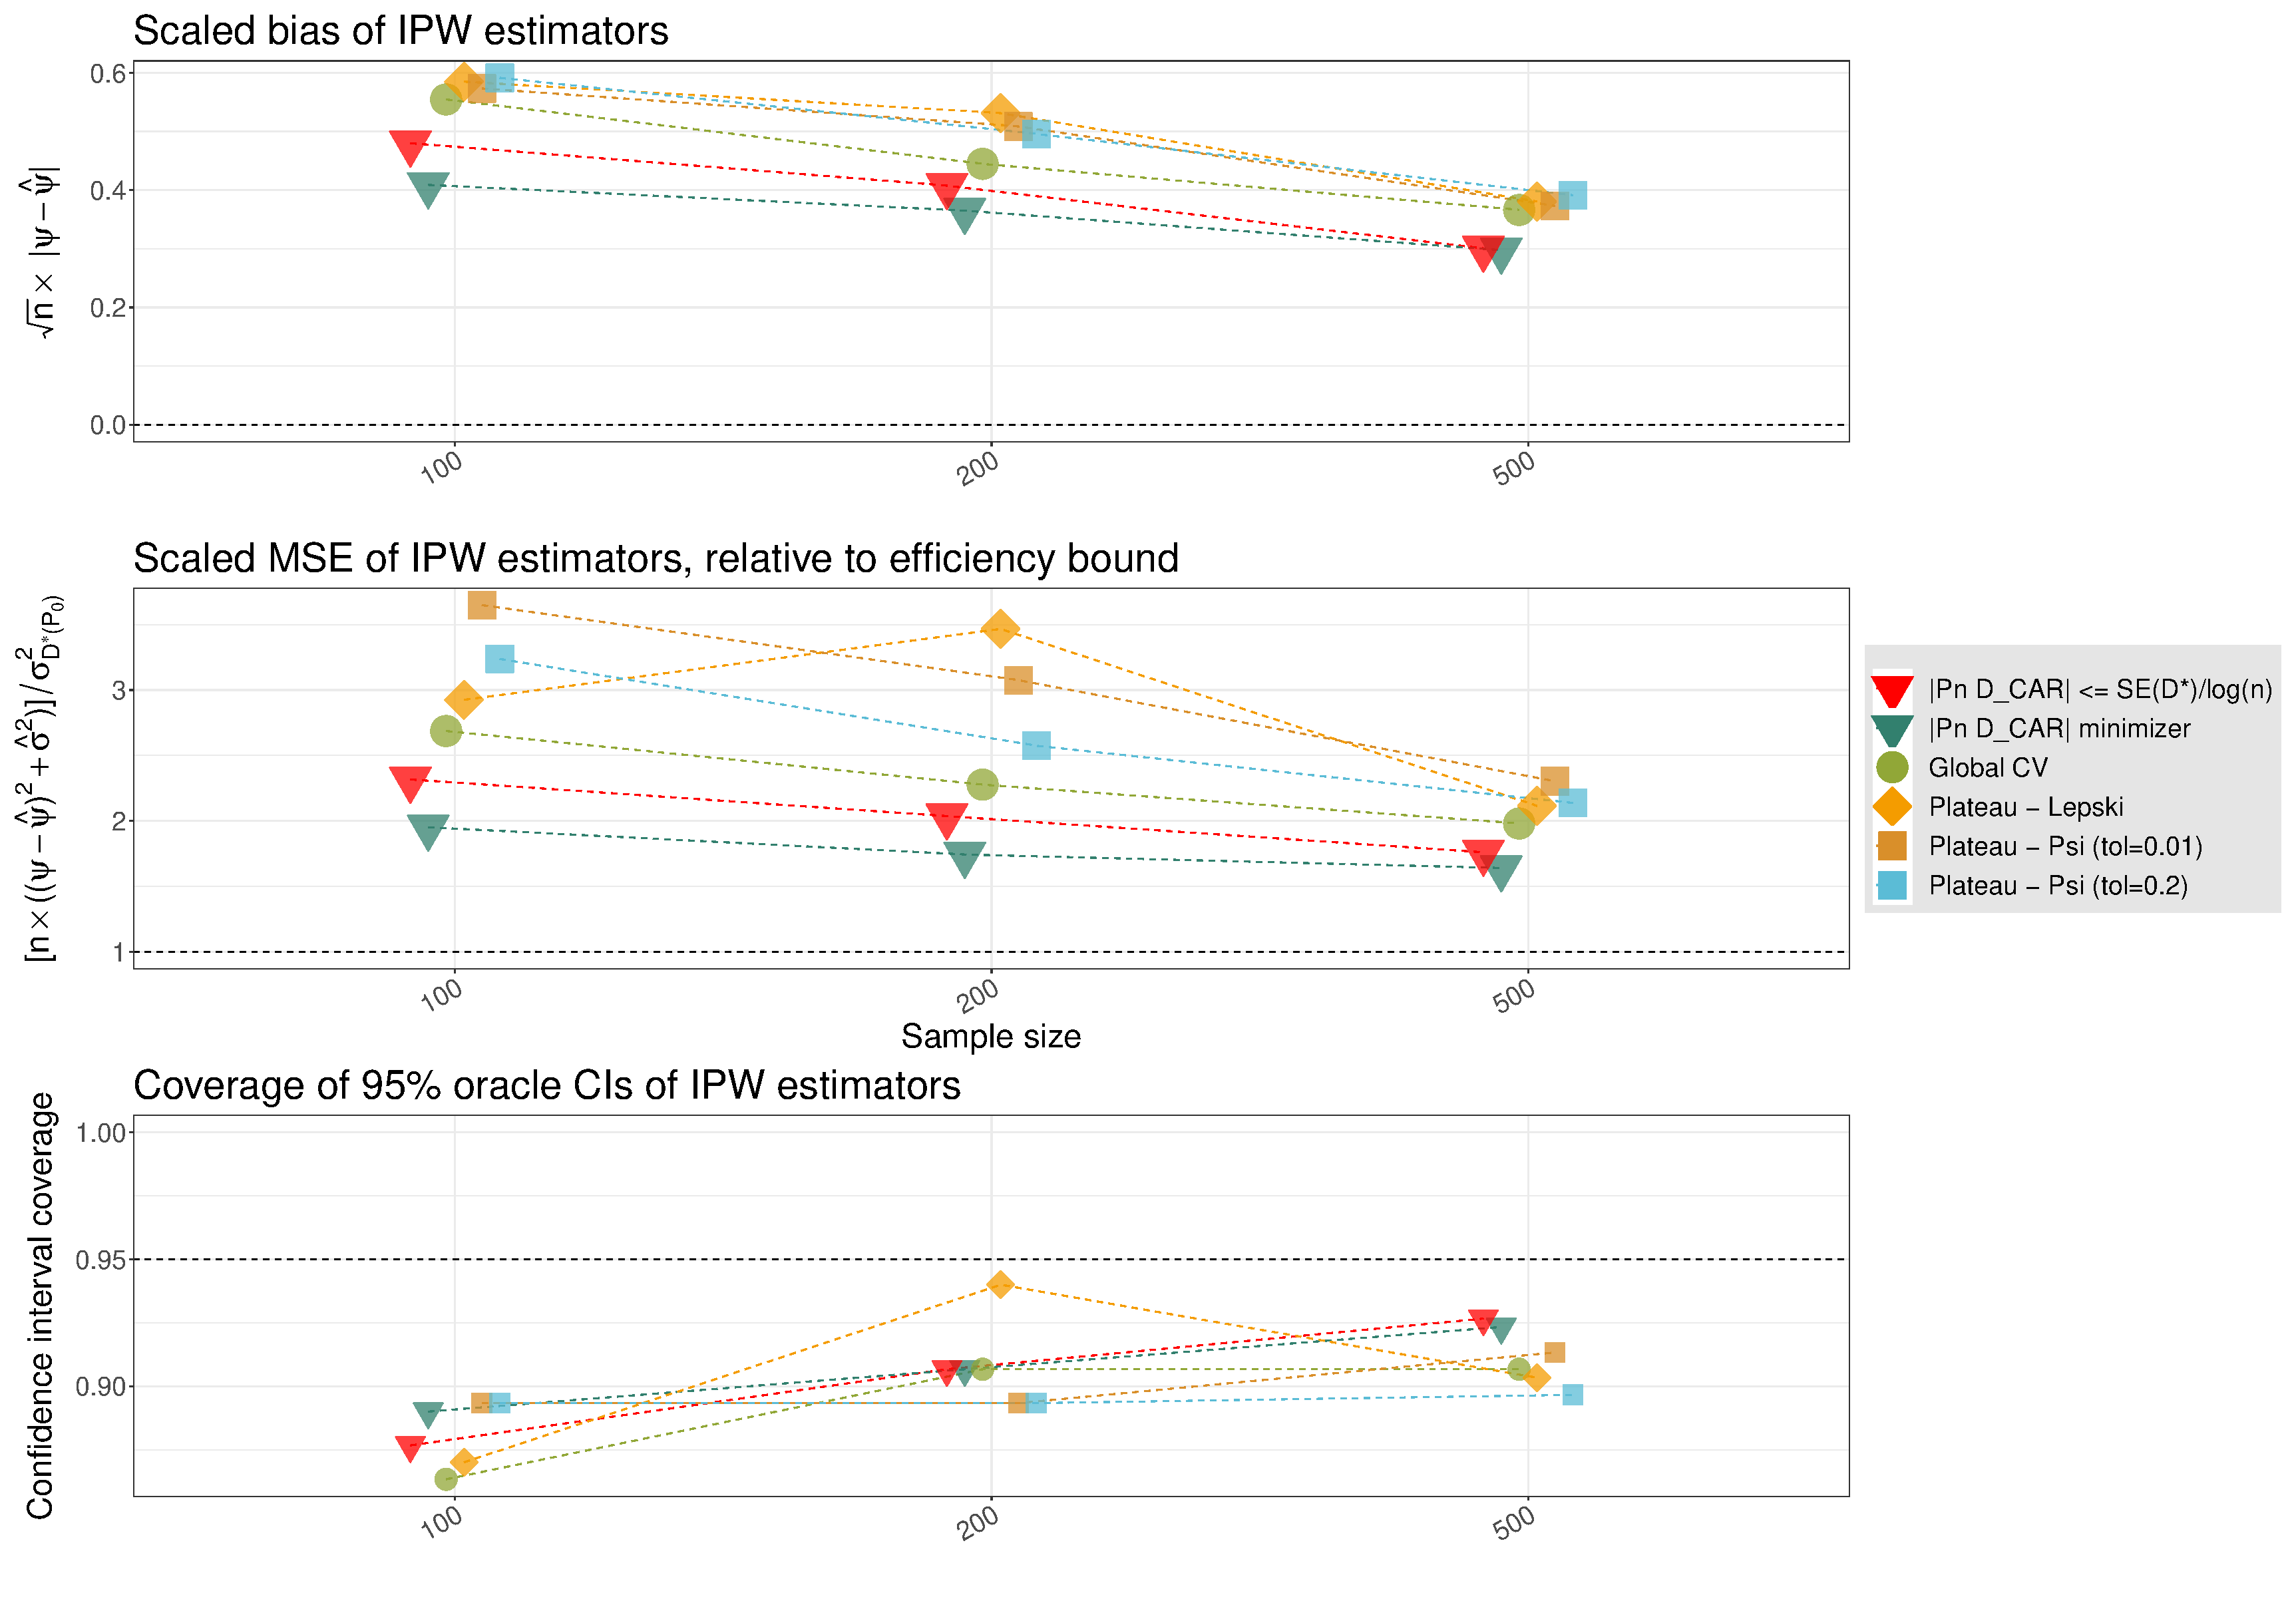
\includegraphics[scale=0.28]{dgp1a_npipw_all_paneled_Qn_hal}
  \caption{Numerical comparisons of nonparametric IPW estimator variants of
     $\psi_{0,\delta}$ for $A \sim \text{Normal}(\mu = f(W), \sigma^2 = k)$.}
  \label{fig:dgp1a_npipw}
\end{figure}
Inspection of Figure~\ref{fig:dgp1a_npipw} reveals generally acceptable
performance of all of our IPW estimators, with bias of $0.06$ and $0.04$ in the
worst and best cases, respectively, at $n=100$; this performance improves to a
bias of $0.018$ in the worst case and of $0.013$ in the best case at $n=500$. In
terms of bias, our IPW estimators using targeted undersmoothing outperform the
other variants uniformly across sample sizes, though the difference is not great
between the best and worst case biases. Considering the scaled MSE, the IPW
estimators using targeted undersmoothing once again dominate the others
uniformly across sample sizes. Notably, in terms of this performance measure,
the IPW estimator utilizing the cross-validation selector outperforms those
using agnostic undersmoothing. This is a surprising finding since
cross-validation chooses the optimal estimator of $g_{0,A}$, not necessarily
that of $\psi_{0,\delta}$; moreover, this relatively good performance suggests
that even cross-validation may make for a reasonably reliable strategy in
constructing nonparametric IPW estimators of $\psi_{0,\delta}$. With respect to
the empirical coverage of oracle confidence intervals, none of the candidate
IPW estimators succeed in attaining the nominal rate, though this is consistent
with the prior observation that none of the estimators are perfectly unbiased at
any of the sample sizes. Altogether, the results of this experiment suggest that
targeted undersmoothing of the HAL generalized propensity score estimator can be
used to construct nonparametric IPW estimators with reasonably good, though not
excellent, asymptotic consistency and efficiency.

\subsection{Simulation \#2: Treatment Mechanism with Unequal Mean and Variance
Dependent on Baseline}\label{hese_sim_norm}

The next scenario is a modification of the previous, in which the form of the
treatment mechanism is kept fixed to a normal distribution, though the mean and
variance are now modified to both be functions of a subset of the baseline
covariates $\{W_1, W_2\}$; $W_3$ has no impact on the treatment mechanism but
does appear in the outcome mechanism, whose forms is a function of the treatment
$A$ and all baseline covariates. Perhaps significantly, the form of the
treatment mechanism in this scenario demands accurate estimation of both the
location and scale parameters of the normal distribution; moreover, the
heteroscedasticity with respect to the baseline covariates complicates accurate
estimation of the conditional density $g_{0,A}$ relative to the form of the
treatment mechanism in the prior scenario. While the form of the outcome
mechanism differs from that in the previous scenario, we again do not expect its
form to affect the construction of our IPW estimators much. The treatment
mechanism takes the form $A \mid W \sim \text{Normal}\left(\mu = W_1 + 2 W_2
- 2 \cdot (1 - W_1) \cdot W_2, \sigma^2 = 2 W_1 + 0.5 (1 - W_1) + W_2 \right)$,
while the outcome mechanism is $Y \mid A, W \sim \text{Bernoulli}\left(p
= \text{expit}(5 (A - 2) + W_1 + 3 W_2^4 - 2 W_3 - \allowbreak 4 (1 - W_1)
W_2)\right)$.

We summarize the performance of our proposed IPW estimators in terms estimation
of $\psi_{0,\delta}$ across the $300$ simulation experiments in
Figure~\ref{fig:dgp1b_npipw}.
\begin{figure}[H]
  \centering
  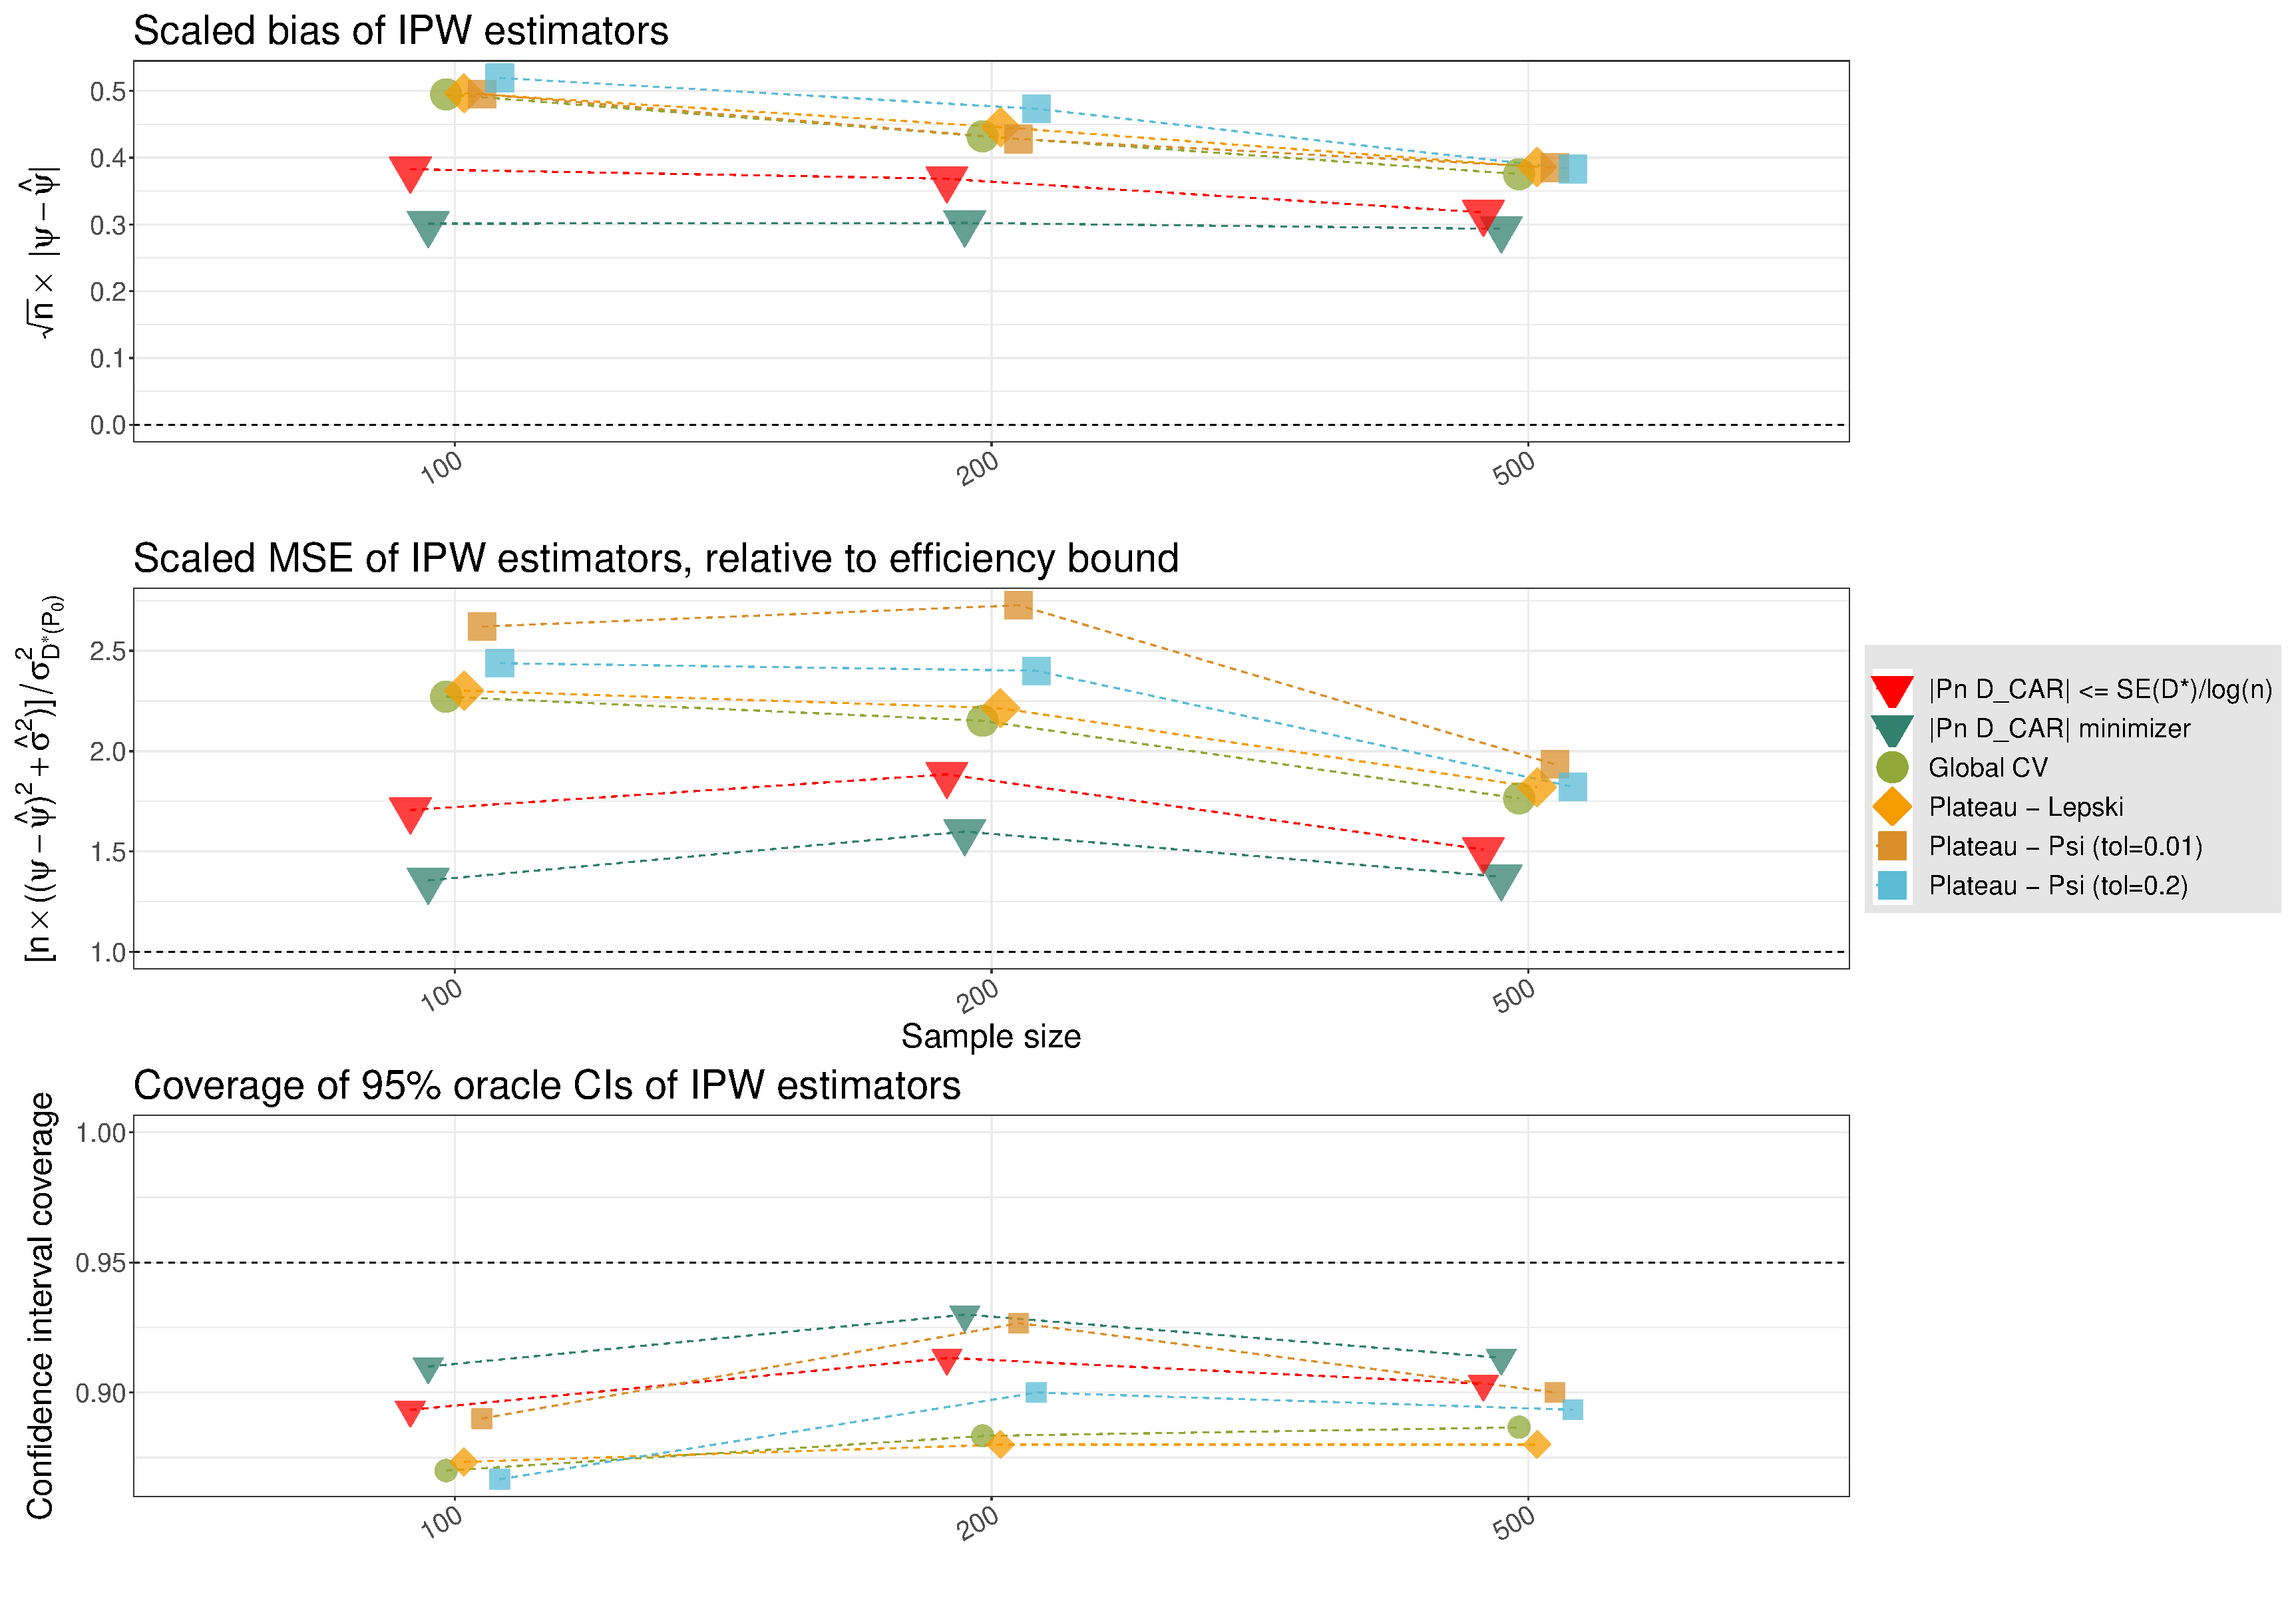
\includegraphics[scale=0.28]{dgp1b_npipw_all_paneled_Qn_hal}
  \caption{Numerical comparisons of nonparametric IPW estimator variants of
     $\psi_{0,\delta}$ for $A \sim \text{Normal}(\mu = f_1(W), \sigma^2 =
     f_2(W))$.}
  \label{fig:dgp1b_npipw}
\end{figure}
Upon examination, Figure~\ref{fig:dgp1b_npipw} reveals relative performance
measures of the IPW estimators very similar to that observed in the prior
scenario. In particular, the IPW estimators constructed based on targeted
undersmoothing outperform all of the other candidates in terms of both bias and
efficiency. In terms of bias, all estimators again achieve acceptable levels of
performance: at $n=100$, bias is $0.052$ in the worst case and $0.03$ in the
best case, while at $n=500$, the same metrics are $0.018$ and $0.013$,
respectively. Turning now to efficiency, none of the estimators achieve the
efficiency bound of the model at the examined sample sizes, though the
decreasing trajectory of their scaled MSEs suggests promising performance at
larger sample sizes. In this scenario, the IPW estimator based on the
cross-validation selector performs similarly to those based on agnostic
undersmoothing. As none of our proposed IPW estimators is perfectly unbiased,
the constructed oracle confidence intervals fail to attain the nominal coverage
rate, consistent with expectations. The results of this experiment echo those of
the first --- our IPW estimators utilizing targeted undersmoothing outperform
the others, though not considerably in any metric.

\subsection{Simulation \#3: Treatment Mechanism with Equal Mean and Variance
Dependent on Baseline}\label{hese_sim_poisson}

We next consider our final experimental scenario, which breaks from the
preceding two examples by basing the form of the treatment mechanism on
a Poisson distribution, so that the mean and variance are both equally impacted
by the relevant baseline covariates. As with the example immediately prior, the
treatment mechanism is a function of a subset of the baseline covariates
$\{W_1, W_2\}$, with $W_3$ only impacting the outcome mechanism. As with our
prior experiments, the form of the outcome mechanism is not expected to impact
our proposed IPW estimators, since estimation of the outcome mechanism only
plays a role in our targeted undersmoothing selection procedures. We note that
the form of the treatment mechanism results in $A$ taking on discrete values in
a fairly large range, unlike the continuous-valued observations that result from
the normal distribution appearing in the prior examples; this treatment
mechanism's form is possibly more compatible with the generalized propensity
score estimator of Algorithm~\ref{alg:pooled_haz_dens}, which utilize
discretization of $A$ for estimation of the conditional density. For this
scenario, the treatment mechanism takes the form $A \mid W \sim
\text{Poisson}\left(\lambda = (1 - W_1) + 0.25 W_2^3 + 2 W_1 W_2 + 4\right)$ and
outcome mechanism is of the form $Y \mid A, W \sim \text{Bernoulli}\left(p
= \text{expit}(A + 2 (1 - W_1) + 0.5 W_2 + 0.5 W_3 + 2 W_1 W_2 - 7)\right)$.

Numerical evaluation of the performance of our proposed IPW estimators of
$\psi_{0,\delta}$ across the $300$ simulation experiments is summarized in
Figure~\ref{fig:dgp2a_npipw}.
\begin{figure}[H]
  \centering
  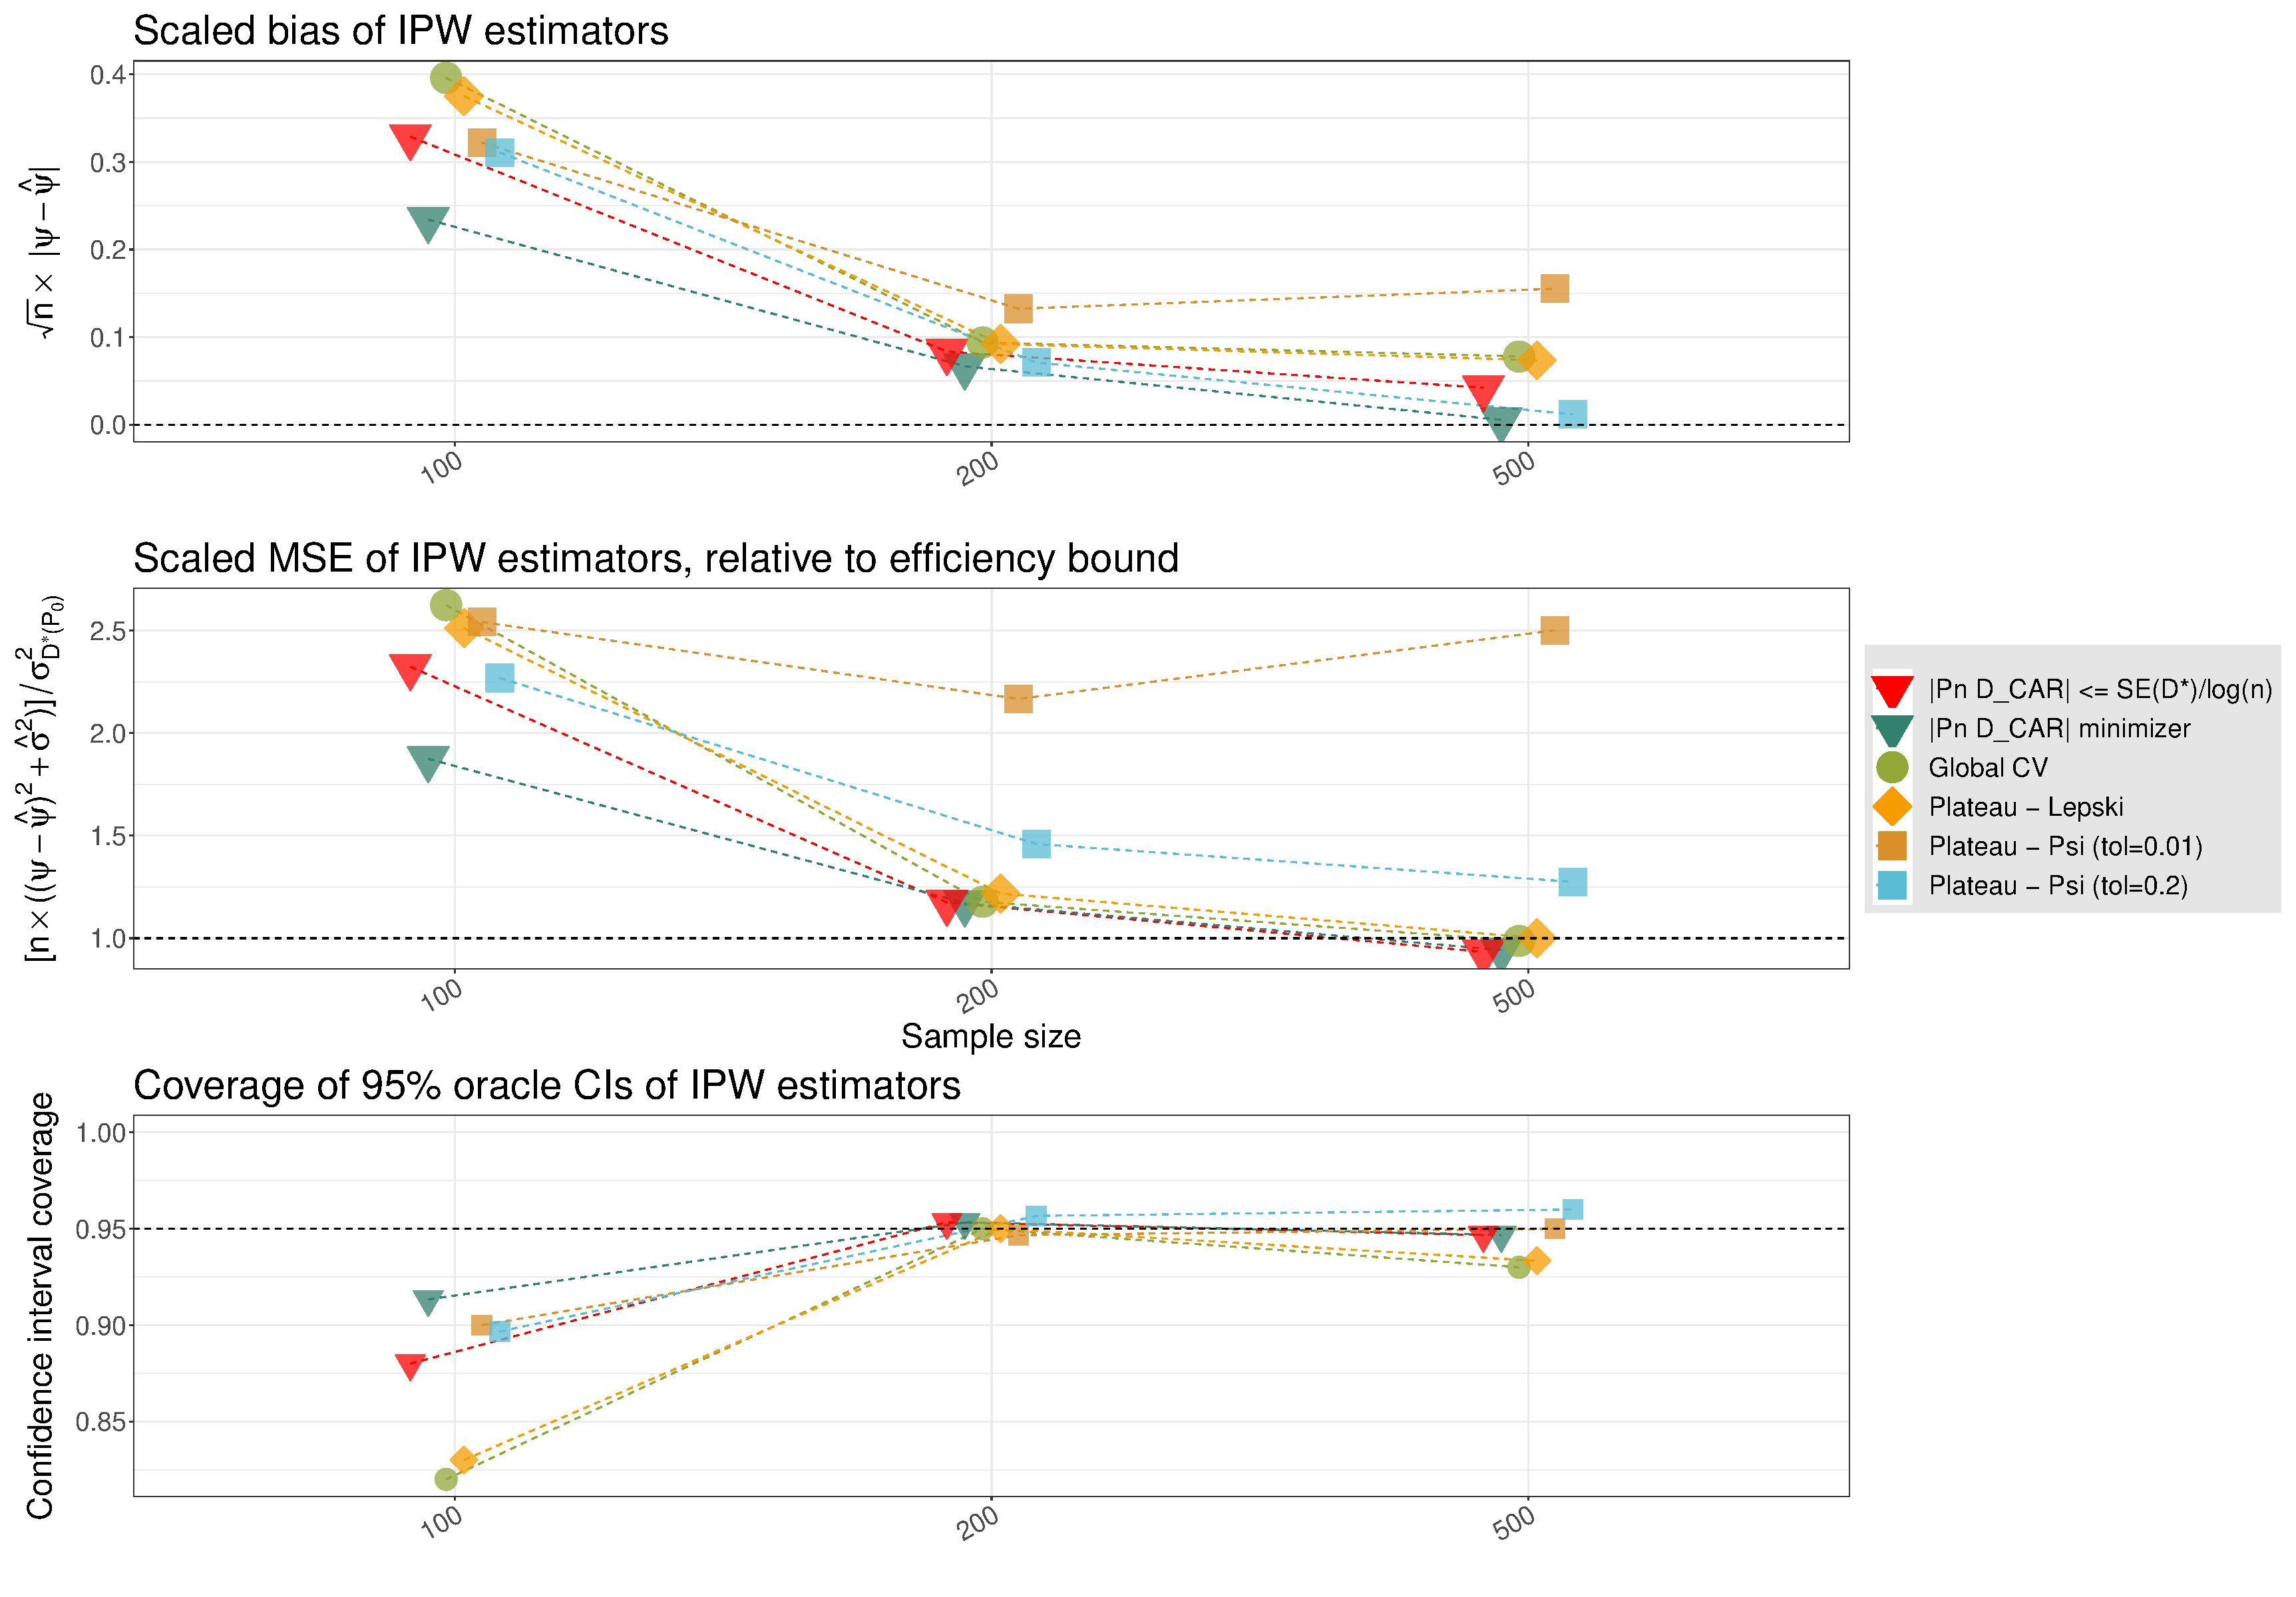
\includegraphics[scale=0.28]{dgp2a_npipw_all_paneled_Qn_hal}
  \caption{Numerical comparisons of nonparametric IPW estimator variants of
       $\psi_{0,\delta}$ for $A \sim \text{Poisson}(\lambda = f(W))$.}
  \label{fig:dgp2a_npipw}
\end{figure}
Figure~\ref{fig:dgp2a_npipw} reveals the best performance of our proposed IPW
estimators encountered thus far. In this setting, the IPW estimator variants
using targeted undersmoothing outperform the others only at the smallest sample
size --- that is, at $n=100$, the IPW estimator based on minimization of the
EIF term arising from Lemma~\ref{lemma:dcar} achieves the lowest bias and best
efficiency. By $n=500$, most estimator variants are nearly unbiased, with the
best performing being IPW estimators minimizing $\lvert P_n D_\text{DCAR}
\rvert$ via targeted undersmoothing and the less restrictive ($\tau = 0.2$)
agnostic undersmoothing selector based on equation~\eqref{eqn:plateau_psi_rel}.
In terms of efficiency, all candidates but the IPW estimators constructed from
agnostic undersmoothing based on equation~\eqref{eqn:plateau_psi_rel} succeed in
achieving the efficiency bound, an excellent level of performance. Notably, even
the IPW estimator based on the cross-validation selector succeeds in this
challenging endeavor, suggesting that it exhibits variance relatively improved
beyond that of the other candidates, on account of the fact that it is not
similarly unbiased. Unlike the prior scenarios, the oracle confidence intervals
of all candidate IPW estimators attain the nominal coverage rate by $n=200$,
with similar performance at $n=500$. Importantly, the excellent performance of
all of the estimator candidates with respect to this metric suggests that all
are capable of providing reliably good performance and that relative performance
differences across the candidates may be better ascribed to variance estimation
than to point estimation, the latter of which is our principal focus. Though the
previously considered scenarios were not discouraging, the results of this set
of experiments are quite positive, suggesting that at least a few variants of
our proposed IPW estimators may successfully applied to reliably and efficiently
estimate $\psi_{0,\delta}$.

%%%%%%%%%%%%%%%%%%%%%%%%%%%%%%%%%%%%%%%%%%%%%%%%%%%%%%%%%%%%%%%%%%%%%%%%%%%%%%%
\section{Discussion}\label{discuss}

The generalized propensity score is a central object in evaluating the causal
effects of continuous treatments. While stochastic interventions provide
a framework for identifying causal effects of realistic interventions, their
formulation too depends on the generalized propensity score. Accordingly,
flexible estimators of this key nuisance quantity, relying on recent
developments in nonparametric regression, are poised to play important roles in
developing consistent and efficient estimators of the causal effects of
stochastic interventions. We have provided an initial examination of the role of
a flexible regression algorithm, the recently developed highly adaptive lasso
estimator, in developing conditional density estimators with favorable
theoretical properties. Building on these contributions, we formulated
nonparametric IPW estimators of the causal effects of stochastic interventions,
previously absent from the causal inference literature. To further improve our
IPW estimators, we outlined several selection procedures, to be used in tandem
with undersmoothing of our proposed HAL-based conditional density estimators, to
allow these novel IPW estimators to achieve the nonparametric efficiency bound,
a property previously attainable by doubly robust estimators. In numerical
experiments, we examined the relative performance our nonparametric IPW
estimators, demonstrating their capability to achieve low bias and attain the
efficiency bound in some examples. Several avenues for future investigation
remain, including potential improvements to doubly robust estimators that
incorporate undersmoothing of the generalized propensity score, which may
exhibit higher-order types of efficiency or make doubly robust
inference~\citep[e.g.,][]{benkeser2017doubly} possible, and the extension of our
nonparametric IPW estimators to more complex settings in which stochastic
interventions have proven useful, including causal mediation
analysis~\citep[e.g.,][]{diaz2020causal}.
